\section{Results}

\subsection{Dataset and baseline reproduction}
Quality control filtering of GLODAP v2.2023 yielded $472{,}530$ high-quality global observations across the four ocean basins (Atlantic: $147{,}448$; Indian: $40{,}391$; Pacific: $187{,}443$; Southern Ocean: $97{,}248$). Figure~\ref{fig:data_overview} illustrates the global sampling distribution in $T$--$S$ space colored by $\tco$. Baseline model fitting confirmed exact reproduction of all primary pipeline results.

\begin{figure}[htbp]
\centering
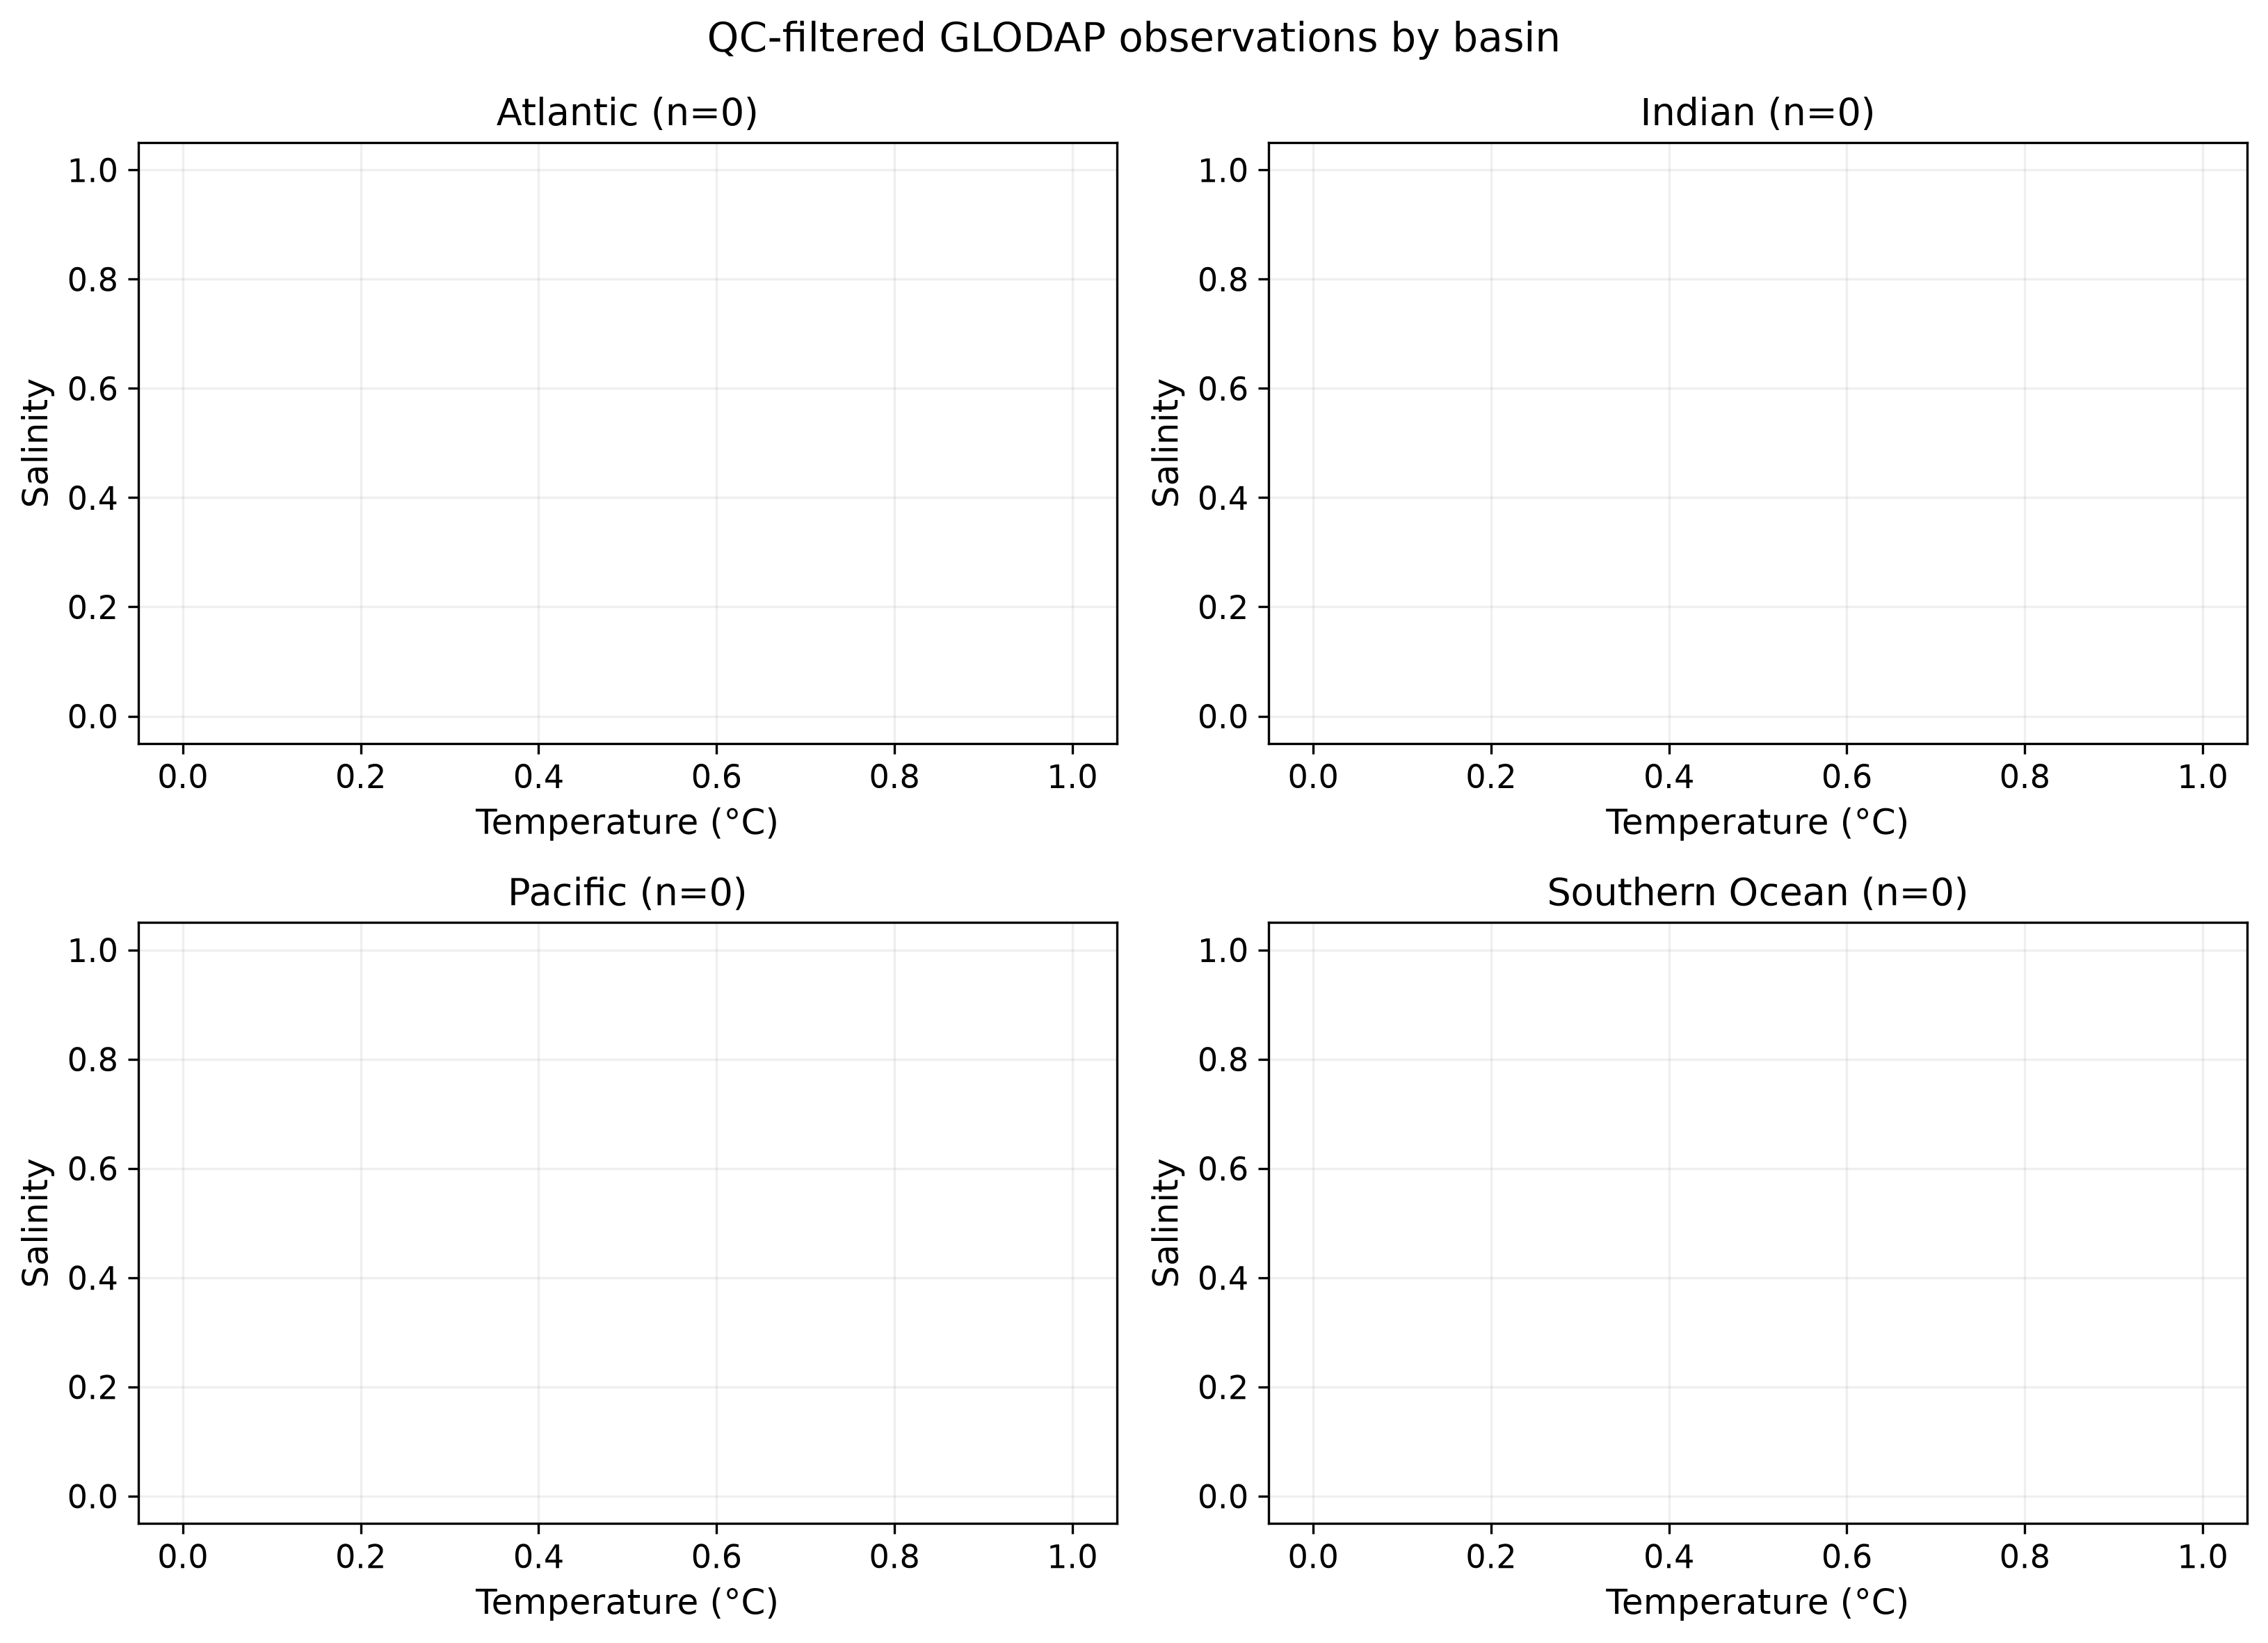
\includegraphics[width=0.95\textwidth]{figures/fig1_data_overview.png}
\caption{Distribution of quality-controlled GLODAP v2.2023 observations across four ocean basins in temperature--salinity space, colored by measured $\tco$ ($\mu\mathrm{mol}\,\mathrm{kg}^{-1}$).}
\label{fig:data_overview}
\end{figure}

\subsection{Model-complexity hierarchy}
Table~\ref{tab:model_hierarchy} and Table~\ref{tab:model_comparison} compare temporal validation performance across the complete model hierarchy. Linear regression ($K=4$) achieves validation RMSEs of $21.59, 14.96, 17.77,$ and $10.66\,\mu\mathrm{mol}\,\mathrm{kg}^{-1}$ in the Atlantic, Indian, Pacific, and Southern Ocean, respectively. Introducing a single quadratic direction in the rank-1 model ($K=5, C=8$) reduces validation RMSE to $20.17, 14.48, 16.00,$ and $10.58\,\mu\mathrm{mol}\,\mathrm{kg}^{-1}$, delivering immediate performance gains over linear models in all basins.

\begin{table}
\caption{Final model hierarchy across temporal validation and external holdout.}
\label{tab:model_hierarchy}
\resizebox{\textwidth}{!}{%
\begin{tabular}{lrrrrrrrrrr}
\toprule
basin & model & parameter\_count & expression\_complexity & validation\_RMSE & validation\_MAE & validation\_R2 & external\_RMSE & external\_MAE & external\_R2 & validation\_delta\_vs\_rank1 \\
\midrule
Atlantic & mean & 1.000 & 1 & 66.879 & 49.937 & -0.017 & 62.940 & 48.806 & -0.001 & 46.708 \\
Atlantic & linear & 4.000 & 4 & 21.591 & 14.666 & 0.894 & 18.538 & 13.134 & 0.913 & 1.419 \\
Atlantic & rank1 & 5.000 & 8 & 20.172 & 14.926 & 0.907 & 17.672 & 13.170 & 0.921 & 0.000 \\
Atlantic & rank2 & 9.000 & 16 & 22.155 & 14.990 & 0.888 & 19.586 & 12.579 & 0.903 & 1.984 \\
Atlantic & full\_quadratic & 10.000 & 20 & 23.406 & 15.570 & 0.875 & 19.621 & 12.528 & 0.903 & 3.235 \\
Atlantic & cubic & 20.000 & 30 & 22.598 & 14.802 & 0.884 & 18.010 & 12.091 & 0.918 & 2.427 \\
Atlantic & frozen\_symbolic & NaN & 15 & 18.998 & 13.292 & 0.918 & 13.125 & 9.502 & 0.956 & -1.174 \\
Indian & mean & 1.000 & 1 & 122.473 & 105.708 & -0.052 & 108.518 & 95.689 & -0.102 & 107.991 \\
Indian & linear & 4.000 & 4 & 14.960 & 11.748 & 0.984 & 19.137 & 14.208 & 0.966 & 0.478 \\
Indian & rank1 & 5.000 & 8 & 14.483 & 11.056 & 0.985 & 18.413 & 13.442 & 0.968 & 0.000 \\
Indian & rank2 & 9.000 & 16 & 14.737 & 11.139 & 0.985 & 18.858 & 13.813 & 0.967 & 0.254 \\
Indian & full\_quadratic & 10.000 & 20 & 13.729 & 10.680 & 0.987 & 14.922 & 11.457 & 0.979 & -0.753 \\
Indian & cubic & 20.000 & 30 & 11.827 & 9.126 & 0.990 & 16.526 & 11.688 & 0.974 & -2.655 \\
Indian & frozen\_symbolic & NaN & 25 & 12.800 & 9.702 & 0.989 & 16.797 & 11.744 & 0.974 & -1.682 \\
Pacific & mean & 1.000 & 1 & 131.396 & 116.426 & -0.001 & 140.892 & 129.001 & -0.046 & 115.394 \\
Pacific & linear & 4.000 & 4 & 17.769 & 13.414 & 0.982 & 17.196 & 13.403 & 0.984 & 1.768 \\
Pacific & rank1 & 5.000 & 8 & 16.002 & 11.089 & 0.985 & 13.821 & 9.636 & 0.990 & 0.000 \\
Pacific & rank2 & 9.000 & 16 & 15.712 & 11.096 & 0.986 & 14.087 & 10.051 & 0.990 & -0.289 \\
Pacific & full\_quadratic & 10.000 & 20 & 15.504 & 10.704 & 0.986 & 14.210 & 9.554 & 0.989 & -0.497 \\
Pacific & cubic & 20.000 & 30 & 14.244 & 9.341 & 0.988 & 12.451 & 8.448 & 0.992 & -1.758 \\
Pacific & frozen\_symbolic & NaN & 20 & 15.488 & 10.706 & 0.986 & 13.531 & 8.995 & 0.990 & -0.514 \\
Southern Ocean & mean & 1.000 & 1 & 59.190 & 50.841 & -0.000 & 51.755 & 47.214 & -0.156 & 48.614 \\
Southern Ocean & linear & 4.000 & 4 & 10.664 & 7.478 & 0.968 & 8.930 & 6.076 & 0.966 & 0.089 \\
Southern Ocean & rank1 & 5.000 & 8 & 10.575 & 7.549 & 0.968 & 8.985 & 5.985 & 0.965 & 0.000 \\
Southern Ocean & rank2 & 9.000 & 16 & 10.540 & 7.607 & 0.968 & 8.895 & 5.985 & 0.966 & -0.035 \\
Southern Ocean & full\_quadratic & 10.000 & 20 & 10.461 & 7.603 & 0.969 & 8.808 & 5.887 & 0.967 & -0.115 \\
Southern Ocean & cubic & 20.000 & 30 & 10.042 & 7.418 & 0.971 & 8.687 & 5.884 & 0.967 & -0.533 \\
Southern Ocean & frozen\_symbolic & NaN & 21 & 9.988 & 7.032 & 0.972 & 8.597 & 5.664 & 0.968 & -0.588 \\
\bottomrule
\end{tabular}%
}
\end{table}

\begin{table}
\caption{Model family comparison. Validation and external holdout metrics.}
\label{tab:model_comparison}
\resizebox{\textwidth}{!}{%
\begin{tabular}{lrrrrrrr}
\toprule
Basin & Model\_name & Parameters & RMSE\_val & MAE\_val & R2\_val & RMSE\_ext & R2\_ext \\
\midrule
Atlantic & Baseline Mean & 1 & 66.879 & 49.937 & -0.017 & 62.940 & -0.001 \\
Atlantic & Linear Regression & 4 & 21.591 & 14.666 & 0.894 & 18.538 & 0.913 \\
Atlantic & Rank-1 Quadratic & 5 & 20.172 & 14.926 & 0.907 & 17.672 & 0.921 \\
Atlantic & Rank-2 Quadratic & 9 & 22.155 & 14.990 & 0.888 & 19.586 & 0.903 \\
Atlantic & Full Second-Order Polynomial & 10 & 23.406 & 15.570 & 0.875 & 19.621 & 0.903 \\
Atlantic & Cubic Polynomial & 20 & 22.598 & 14.802 & 0.884 & 18.010 & 0.918 \\
Indian & Baseline Mean & 1 & 122.473 & 105.708 & -0.052 & 108.518 & -0.102 \\
Indian & Linear Regression & 4 & 14.960 & 11.748 & 0.984 & 19.137 & 0.966 \\
Indian & Rank-1 Quadratic & 5 & 14.483 & 11.056 & 0.985 & 18.413 & 0.968 \\
Indian & Rank-2 Quadratic & 9 & 14.737 & 11.139 & 0.985 & 18.858 & 0.967 \\
Indian & Full Second-Order Polynomial & 10 & 13.729 & 10.680 & 0.987 & 14.922 & 0.979 \\
Indian & Cubic Polynomial & 20 & 11.827 & 9.126 & 0.990 & 16.526 & 0.974 \\
Pacific & Baseline Mean & 1 & 131.396 & 116.426 & -0.001 & 140.892 & -0.046 \\
Pacific & Linear Regression & 4 & 17.769 & 13.414 & 0.982 & 17.196 & 0.984 \\
Pacific & Rank-1 Quadratic & 5 & 16.002 & 11.089 & 0.985 & 13.821 & 0.990 \\
Pacific & Rank-2 Quadratic & 9 & 15.712 & 11.096 & 0.986 & 14.087 & 0.990 \\
Pacific & Full Second-Order Polynomial & 10 & 15.504 & 10.704 & 0.986 & 14.210 & 0.989 \\
Pacific & Cubic Polynomial & 20 & 14.244 & 9.341 & 0.988 & 12.451 & 0.992 \\
Southern Ocean & Baseline Mean & 1 & 59.190 & 50.841 & -0.001 & 51.755 & -0.156 \\
Southern Ocean & Linear Regression & 4 & 10.664 & 7.478 & 0.968 & 8.930 & 0.966 \\
Southern Ocean & Rank-1 Quadratic & 5 & 10.575 & 7.549 & 0.968 & 8.985 & 0.965 \\
Southern Ocean & Rank-2 Quadratic & 9 & 10.540 & 7.607 & 0.968 & 8.895 & 0.966 \\
Southern Ocean & Full Second-Order Polynomial & 10 & 10.461 & 7.603 & 0.969 & 8.808 & 0.967 \\
Southern Ocean & Cubic Polynomial & 20 & 10.042 & 7.418 & 0.971 & 8.687 & 0.967 \\
\bottomrule
\end{tabular}%
}
\end{table}


\begin{figure}[htbp]
\centering
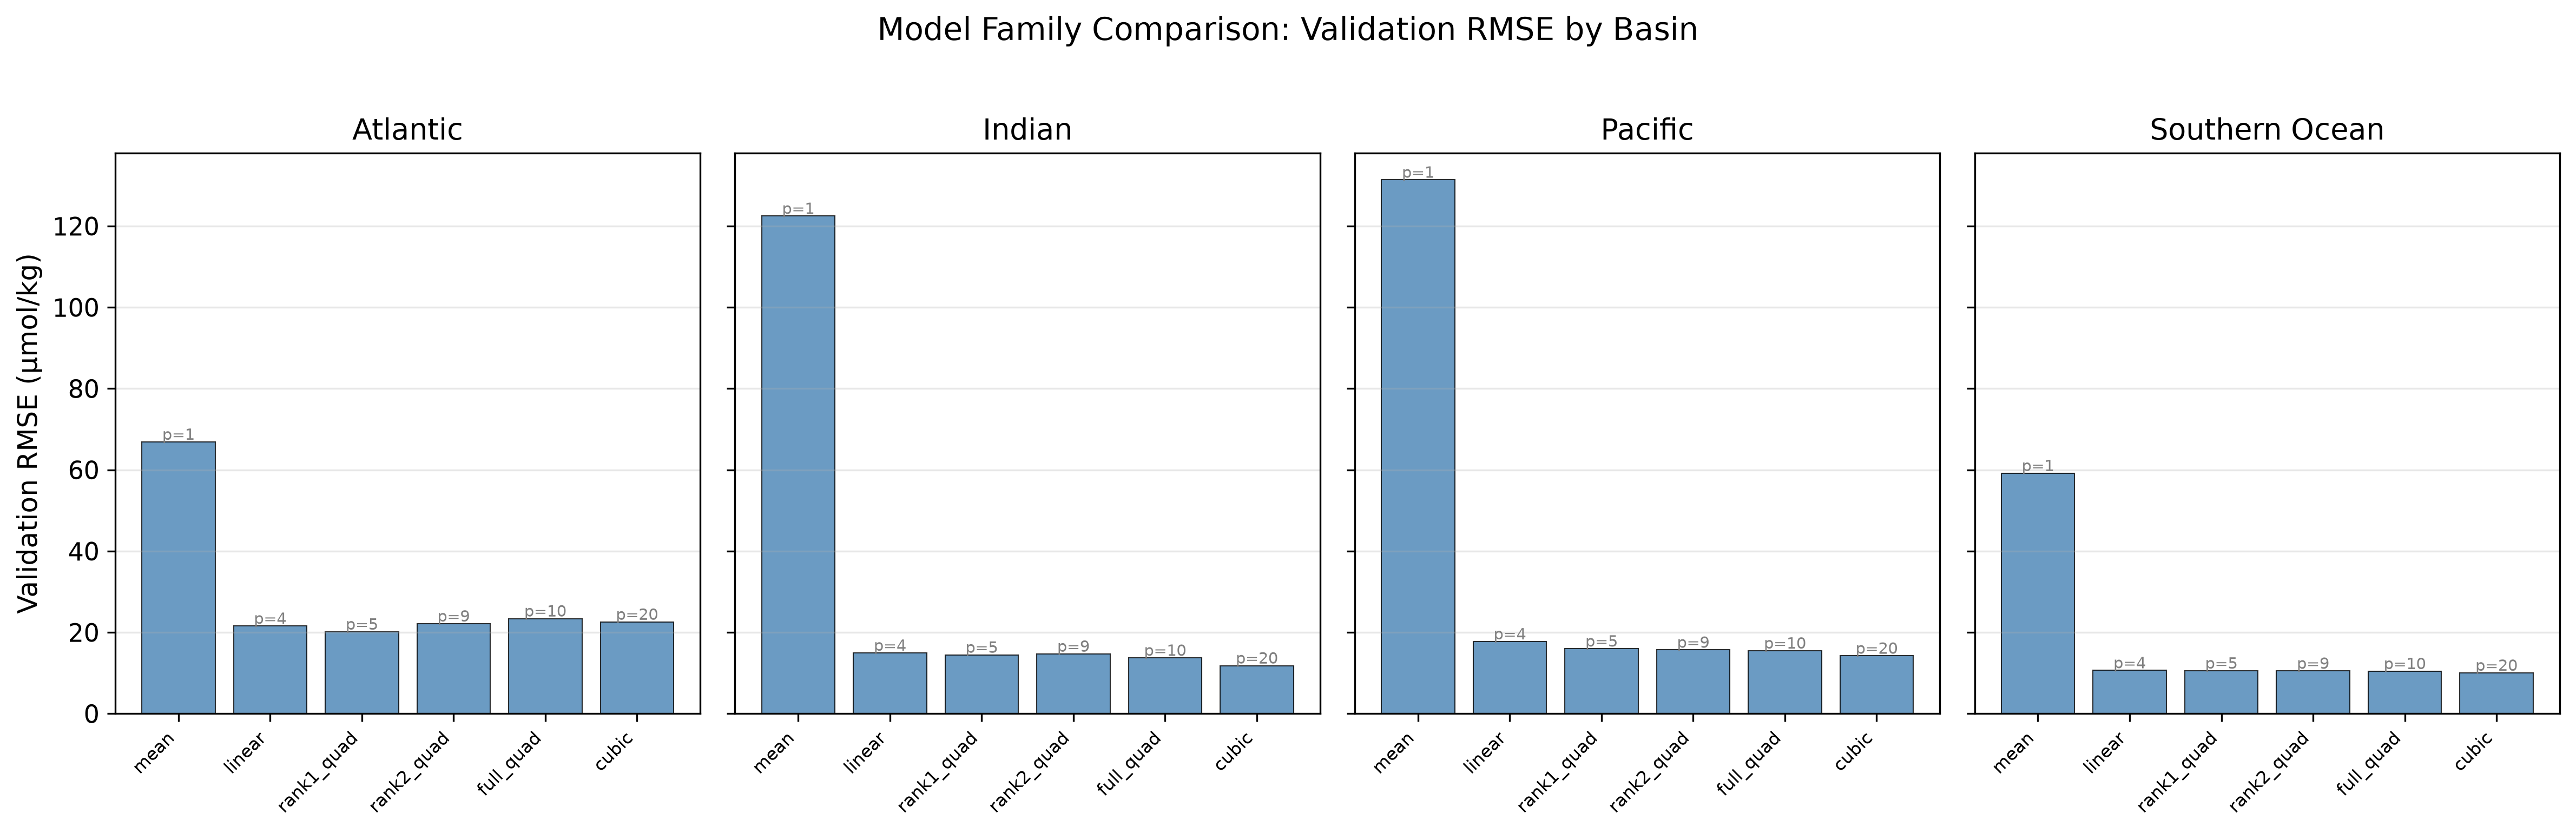
\includegraphics[width=0.95\textwidth]{figures/fig2_model_comparison.png}
\caption{Temporal validation RMSE across the predefined model hierarchy. Parameter count ($K$) is indicated above each bar.}
\label{fig:model_hierarchy}
\end{figure}

\subsection{Symbolic-regression candidate recurrence}
Across the 48 PySR evolutionary searches, a total of 599 candidate expressions were retained, of which 252 entries lay on basin-specific Pareto frontiers. Structurally, 86 expressions belonged to the rank-1 quadratic family. Rank-1 candidates recurred in 24 of the 48 search cells (50.0\% cell-level recurrence), appearing in all four ocean basins.

However, recurrence exhibited strong operator-space dependence (Table~\ref{tab:recurrence} and Figure~\ref{fig:recurrence}). In the Atlantic Ocean, rank-1 candidates were recovered exclusively in Search C ($+,-,\times,\div,(\cdot)^2,\sqrt{\cdot}$), where explicit squaring operators were available. In basic arithmetic (Search A) and exponential/logarithmic spaces (Search B), PySR failed to discover rank-1 quadratic expressions in the Atlantic. This confirms that symbolic recovery depends on operator space parameterization.

{\small
\begin{table}[htbp]
\centering
\caption{Symbolic-regression library and rank-1 recurrence. A cell is a basin $\times$ operator-space $\times$ seed combination. Rank-1 counts use the heuristic family classifier and are not algebraically deduplicated.}
\label{tab:recurrence}
\begin{tabular}{lr}
\toprule
Quantity & Value \\
\midrule
Completed searches & 48 \\
Extracted/evaluated candidates & 599 \\
Pareto-optimal entries & 252 \\
Rank-1 classified candidates & 86 \\
Cells with $\ge 1$ rank-1 candidate & 24/48 \\
Basins with rank-1 recovery & 4/4 \\
Atlantic cells with rank-1 & 3/12 (Search C only) \\
Indian cells with rank-1 & 7/12 \\
Pacific cells with rank-1 & 5/12 \\
Southern Ocean cells with rank-1 & 9/12 \\
\bottomrule
\end{tabular}
\end{table}

}

\begin{figure}[htbp]
\centering
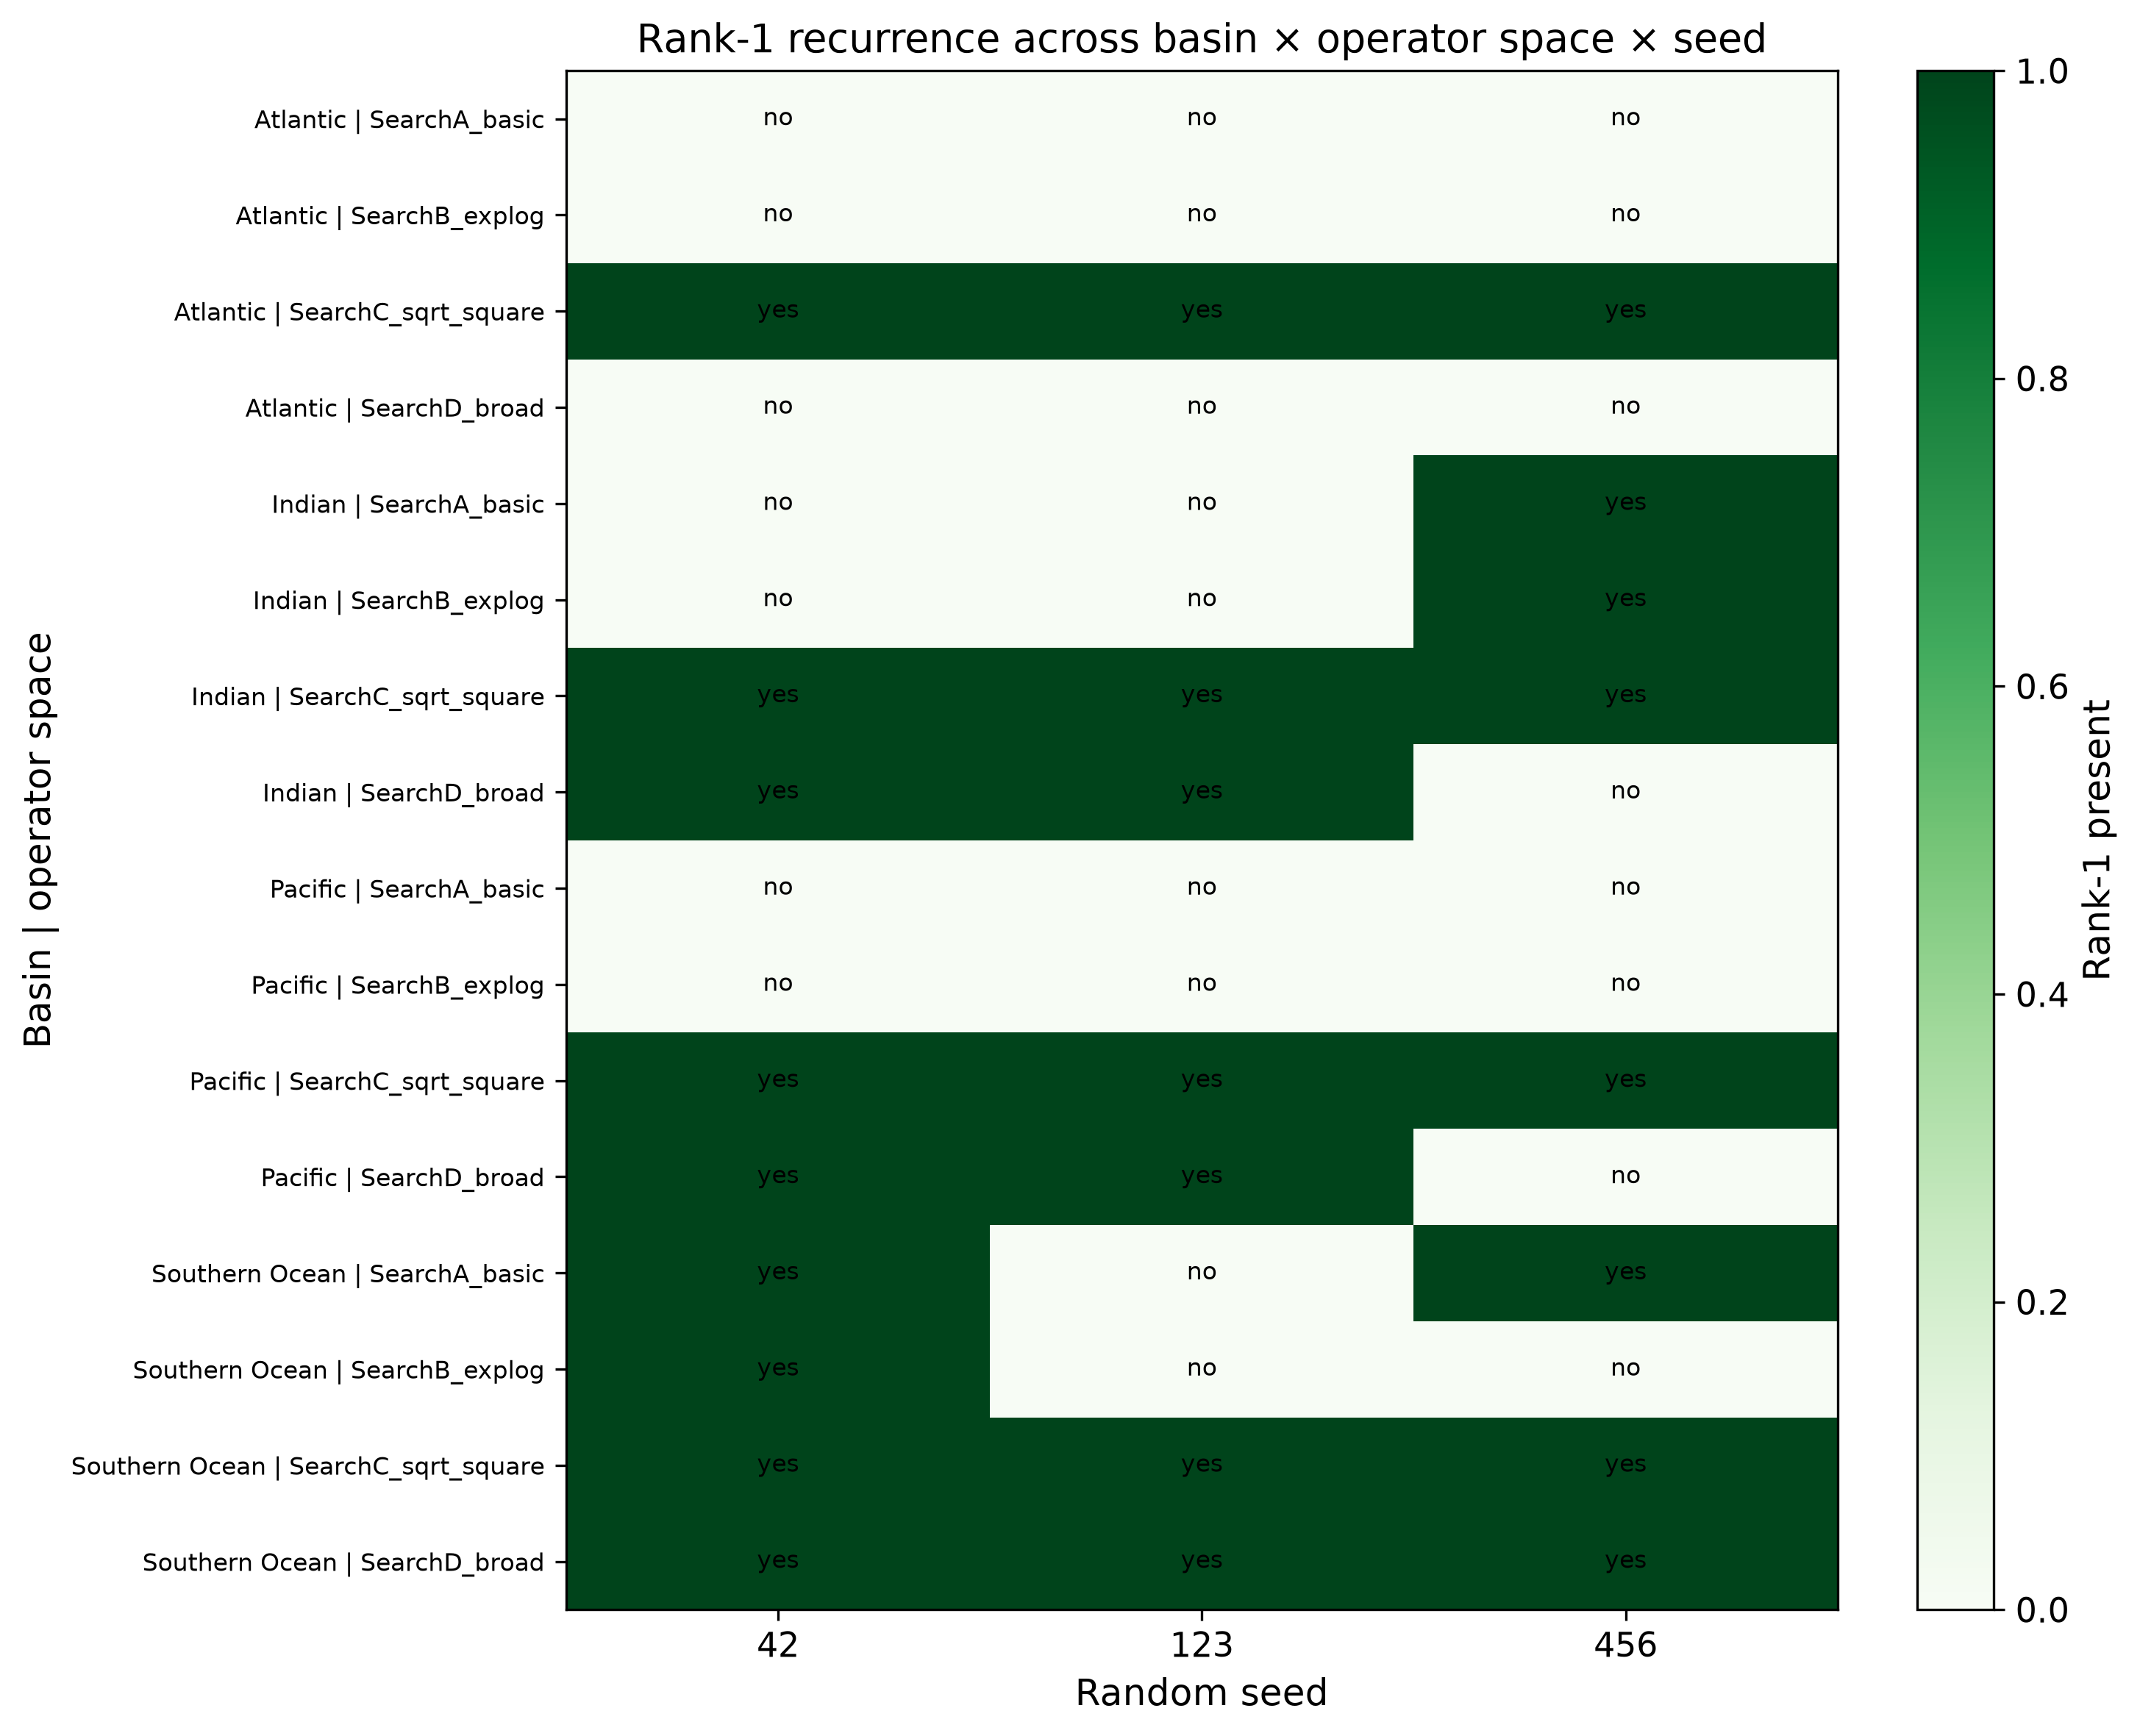
\includegraphics[width=0.95\textwidth]{figures/fig4_rank1_recurrence.png}
\caption{Rank-1 recurrence across 48 search cells ($4\text{ basins} \times 4\text{ operator sets} \times 3\text{ random seeds}$). Green cells indicate successful recovery of rank-1 candidates.}
\label{fig:recurrence}
\end{figure}

\subsection{Pareto frontier and accuracy/complexity tradeoff}
Figure~\ref{fig:pareto_frontier} presents the empirical Pareto frontiers of validation RMSE versus PySR expression complexity ($C$). Higher-complexity symbolic expressions achieve the lowest raw validation RMSE in all basins (Atlantic: $19.00\,\mu\mathrm{mol}\,\mathrm{kg}^{-1}$ at $C=15$; Indian: $12.80\,\mu\mathrm{mol}\,\mathrm{kg}^{-1}$ at $C=25$; Pacific: $15.49\,\mu\mathrm{mol}\,\mathrm{kg}^{-1}$ at $C=20$; Southern Ocean: $9.99\,\mu\mathrm{mol}\,\mathrm{kg}^{-1}$ at $C=21$).

However, as shown in Table~\ref{tab:pareto_summary}, these 3--12\% RMSE improvements require two- to three-fold higher expression complexity. The rank-1 quadratic ($K=5, C=8$) occupies the low-complexity portion of the Pareto frontier. Across strict 1\%, 2\%, and 5\% accuracy tolerance thresholds, rank-1 satisfies the 5\% tolerance threshold only in the Pacific Ocean, confirming that rank-1 is an efficient low-complexity approximation rather than a universal Pareto knee.

\begin{table}
\caption{Pareto-frontier summaries and tolerance thresholds.}
\label{tab:pareto_summary}
\resizebox{\textwidth}{!}{%
\begin{tabular}{lrrrrrrrr}
\toprule
basin & best\_RMSE & best\_complexity & rank1\_RMSE & rank1\_complexity & tolerance & simplest\_within\_tolerance\_RMSE & simplest\_within\_tolerance\_complexity & rank1\_within\_tolerance \\
\midrule
Atlantic & 18.998 & 15 & 20.172 & 8 & 0.010 & 19.041 & 13 & False \\
Atlantic & 18.998 & 15 & 20.172 & 8 & 0.020 & 19.041 & 13 & False \\
Atlantic & 18.998 & 15 & 20.172 & 8 & 0.050 & 19.041 & 13 & False \\
Indian & 12.800 & 25 & 14.483 & 8 & 0.010 & 12.800 & 25 & False \\
Indian & 12.800 & 25 & 14.483 & 8 & 0.020 & 12.963 & 24 & False \\
Indian & 12.800 & 25 & 14.483 & 8 & 0.050 & 13.095 & 20 & False \\
Pacific & 15.488 & 20 & 16.002 & 8 & 0.010 & 15.488 & 20 & False \\
Pacific & 15.488 & 20 & 16.002 & 8 & 0.020 & 15.488 & 20 & False \\
Pacific & 15.488 & 20 & 16.002 & 8 & 0.050 & 16.198 & 15 & True \\
Southern Ocean & 9.988 & 21 & 10.575 & 8 & 0.010 & 10.080 & 20 & False \\
Southern Ocean & 9.988 & 21 & 10.575 & 8 & 0.020 & 10.126 & 15 & False \\
Southern Ocean & 9.988 & 21 & 10.575 & 8 & 0.050 & 10.429 & 12 & False \\
\bottomrule
\end{tabular}%
}
\end{table}


\begin{figure}[htbp]
\centering
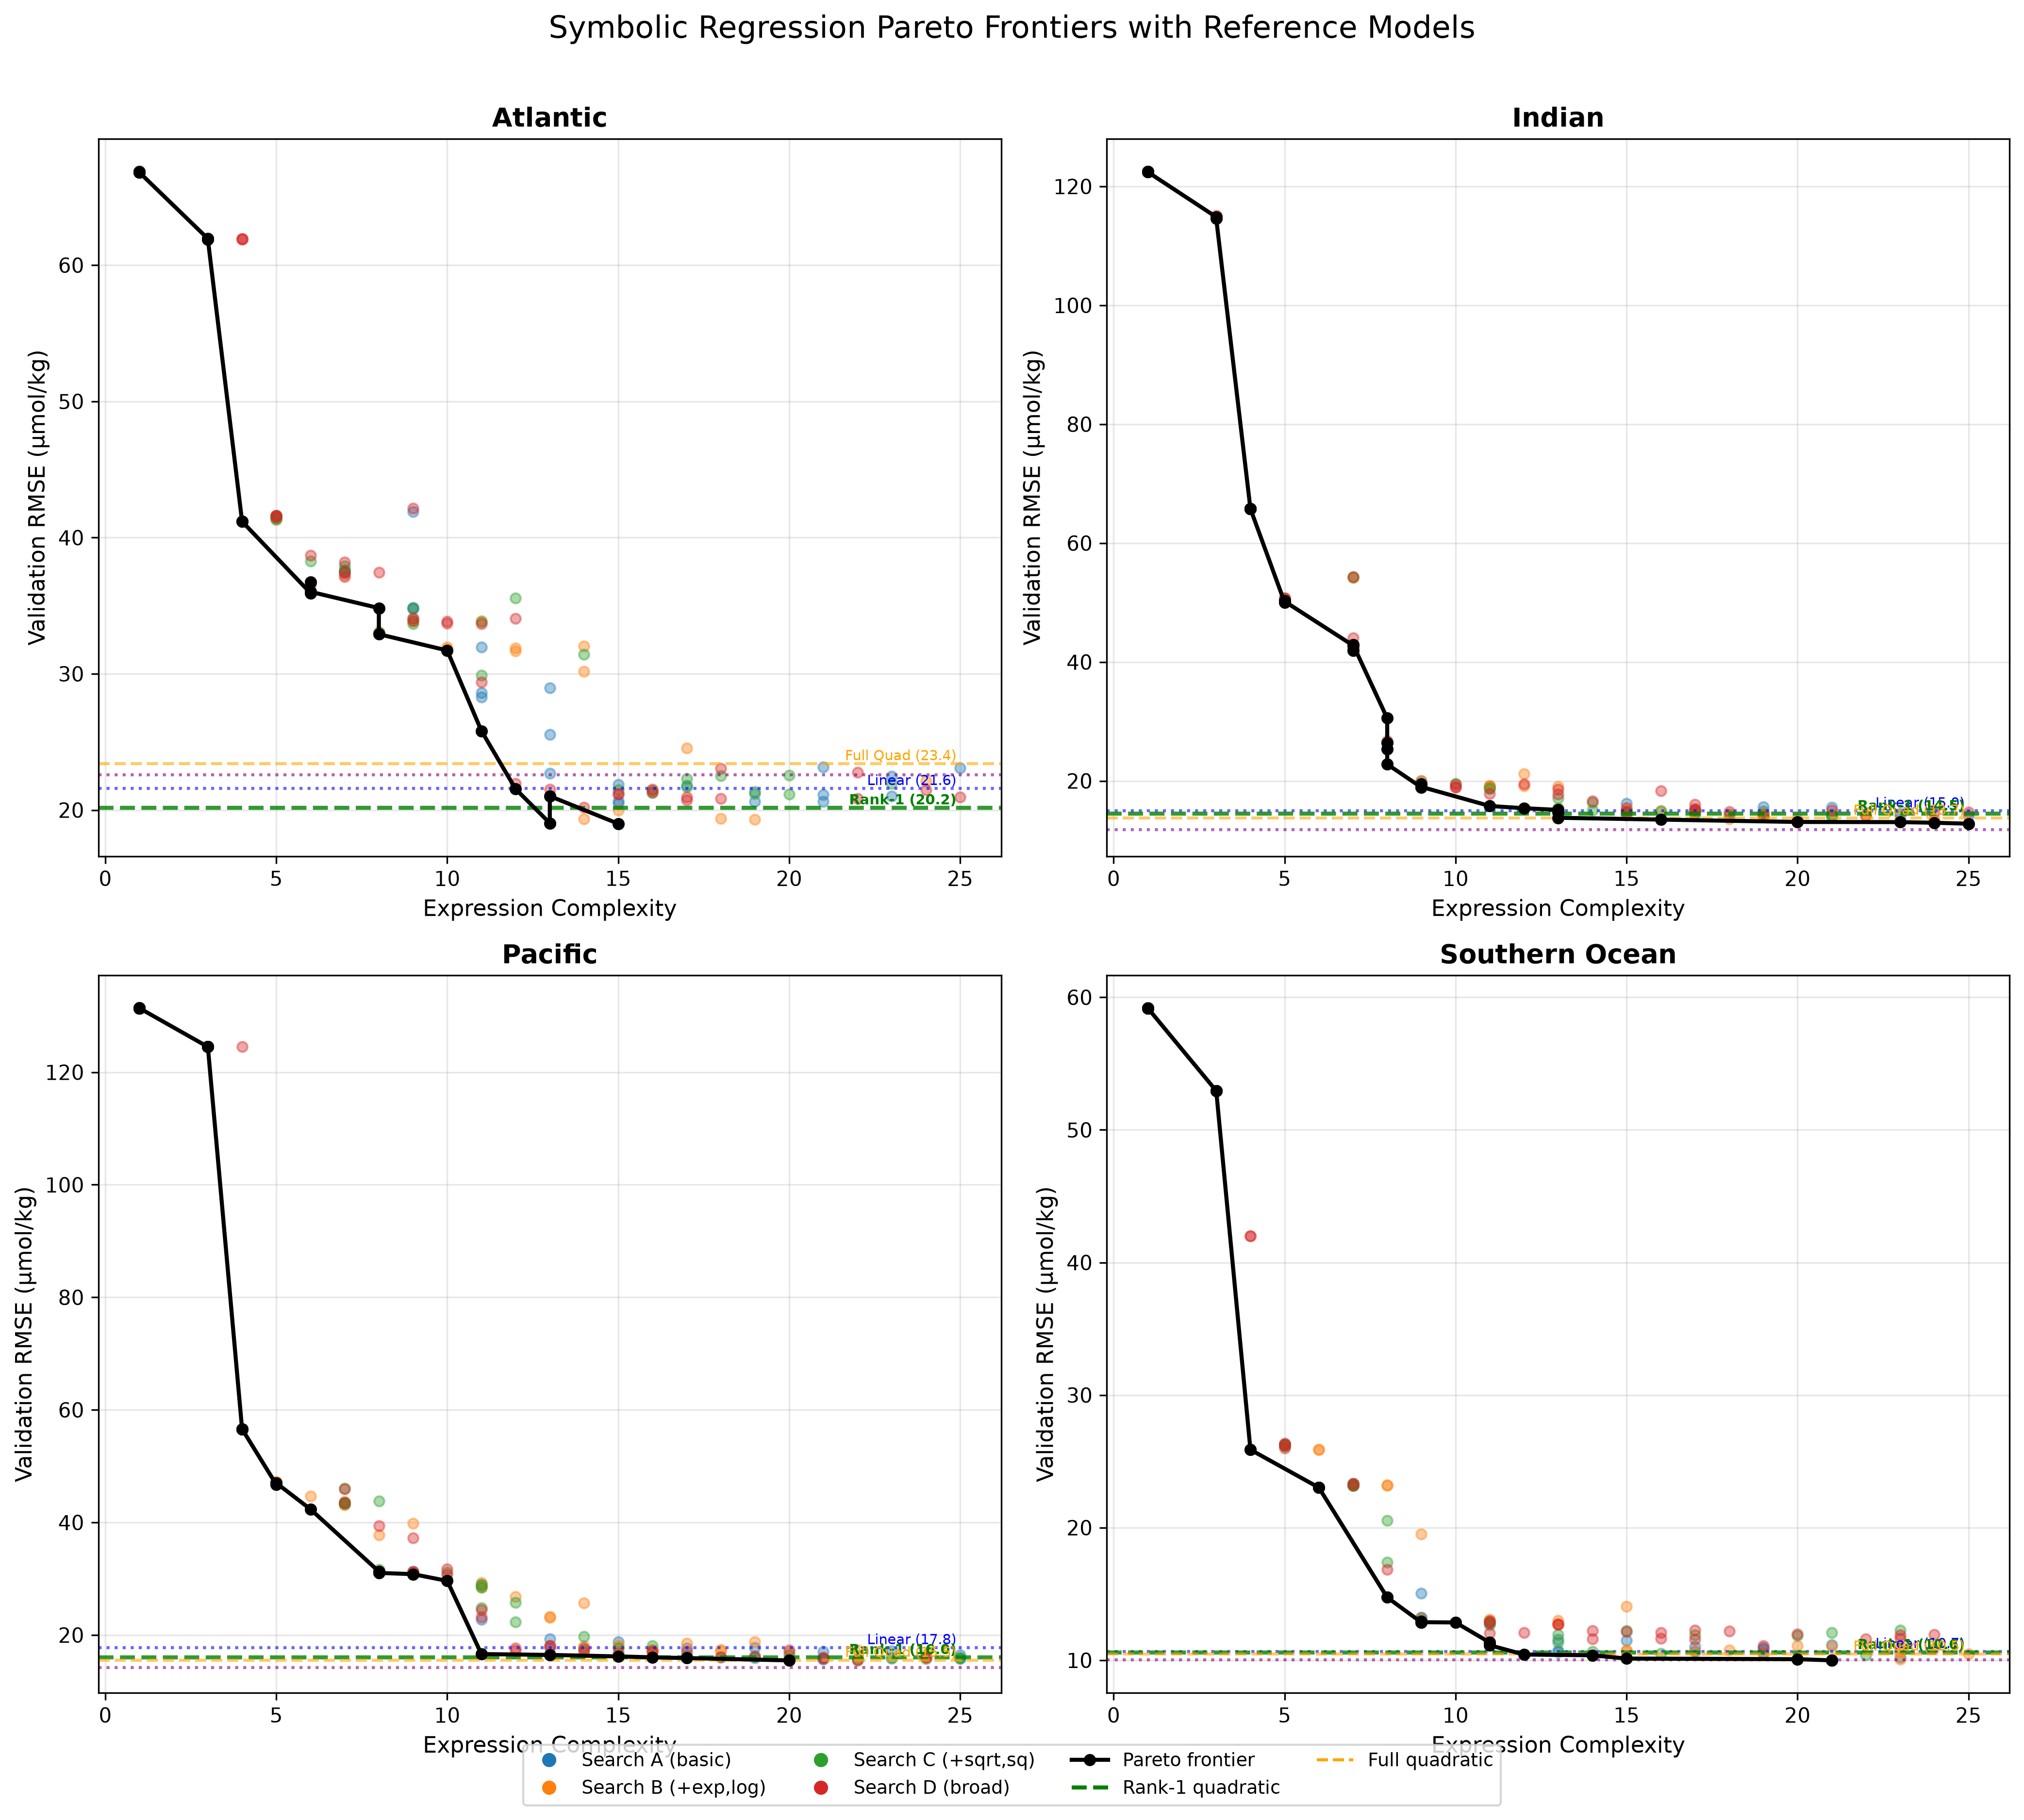
\includegraphics[width=0.95\textwidth]{figures/fig1_pareto_frontier_final.png}
\caption{Empirical Pareto frontiers of validation RMSE versus PySR expression complexity ($C$). The rank-1 quadratic model ($C=8$) is highlighted relative to symbolic candidates and classical baseline models.}
\label{fig:pareto_frontier}
\end{figure}

\subsection{Rank-1 versus rank-2 quadratic comparison}
A central structural finding of this study is the comparison between rank-1 ($K=5$) and rank-2 ($K=9$) quadratic models. Adding a second quadratic direction ($z_2^2$) provides no meaningful predictive benefit:
\begin{itemize}[nosep]
\item \textbf{Atlantic}: Rank-2 validation RMSE increases by $+1.98\,\mu\mathrm{mol}\,\mathrm{kg}^{-1}$ ($22.16$ vs.\ $20.17$), indicating overfitting.
\item \textbf{Indian}: Rank-2 validation RMSE increases by $+0.25\,\mu\mathrm{mol}\,\mathrm{kg}^{-1}$ ($14.74$ vs.\ $14.48$).
\item \textbf{Pacific}: Rank-2 validation RMSE decreases marginally by $-0.29\,\mu\mathrm{mol}\,\mathrm{kg}^{-1}$ ($15.71$ vs.\ $16.00$).
\item \textbf{Southern Ocean}: Rank-2 validation RMSE decreases negligibly by $-0.04\,\mu\mathrm{mol}\,\mathrm{kg}^{-1}$ ($10.54$ vs.\ $10.58$).
\end{itemize}
This result demonstrates that quadratic curvature in empirical $\tco$ predictor space is essentially one-dimensional.

\subsection{Comparison with full quadratic and cubic models}
The full quadratic model ($K=10$) fits all 10 unconstrained second-order coefficients. In the Atlantic, rank-1 ($20.17\,\mu\mathrm{mol}\,\mathrm{kg}^{-1}$) outperforms full quadratic ($23.41\,\mu\mathrm{mol}\,\mathrm{kg}^{-1}$) by $13.8\%$ due to unconstrained polynomial overfitting in data-sparse boundary regions. In the Indian, Pacific, and Southern Ocean, full quadratic improves upon rank-1 by small margins ($0.75, 0.50,$ and $0.12\,\mu\mathrm{mol}\,\mathrm{kg}^{-1}$, respectively). Cubic models ($K=20$) yield further modest reductions ($11.83, 14.24, 10.04\,\mu\mathrm{mol}\,\mathrm{kg}^{-1}$) at four times the parameter cost of rank-1.

\subsection{Temporal generalization}
Temporal out-of-sample performance was evaluated on the temporal validation set ($2015$--$2017$). The rank-1 model maintained consistent performance without temporal degradation, achieving validation $R^2$ values of $0.907$ (Atlantic), $0.985$ (Indian), $0.985$ (Pacific), and $0.968$ (Southern Ocean).

\subsection{Spatial and cruise generalization}
Table~\ref{tab:spatial_validation} reports out-of-sample performance under spatial-block ($5^\circ \times 10^\circ$) and cruise-blocked GroupKFold cross-validation on pre-2018 data. Spatial-blocked rank-1 RMSEs were $16.30\,\mu\mathrm{mol}\,\mathrm{kg}^{-1}$ (Atlantic), $16.61\,\mu\mathrm{mol}\,\mathrm{kg}^{-1}$ (Indian), $16.03\,\mu\mathrm{mol}\,\mathrm{kg}^{-1}$ (Pacific), and $9.16\,\mu\mathrm{mol}\,\mathrm{kg}^{-1}$ (Southern Ocean). Cruise-blocked rank-1 RMSEs were $16.91, 17.39, 16.03,$ and $9.22\,\mu\mathrm{mol}\,\mathrm{kg}^{-1}$.

While rank-1 maintains low generalization error under blocked sampling, model rankings change across validation regimes. For example, in Atlantic spatial validation, rank-2 ($15.46\,\mu\mathrm{mol}\,\mathrm{kg}^{-1}$) and full quadratic ($15.55\,\mu\mathrm{mol}\,\mathrm{kg}^{-1}$) achieve lower RMSE than rank-1 ($16.30\,\mu\mathrm{mol}\,\mathrm{kg}^{-1}$), demonstrating that model ranking is regime-dependent.

\begin{longtable}{lrrrrrr}
\caption{Spatial- and cruise-blocked validation summary. Full fold diagnostics are in the CSV output.} \label{tab:spatial_validation} \\
\toprule
Basin & Block & Model & Groups & RMSE & RMSE SD & R2 \\
\midrule
\endfirsthead
\caption[]{Spatial- and cruise-blocked validation summary. Full fold diagnostics are in the CSV output.} \\
\toprule
Basin & Block & Model & Groups & RMSE & RMSE SD & R2 \\
\midrule
\endhead
\midrule
\multicolumn{7}{r}{Continued on next page} \\
\midrule
\endfoot
\bottomrule
\endlastfoot
Atlantic & cruise & frozen\_symbolic & 192 & 17.519 & 4.689 & 0.893 \\
Atlantic & cruise & full\_quadratic & 192 & 15.629 & 2.777 & 0.914 \\
Atlantic & cruise & linear & 192 & 16.667 & 4.336 & 0.903 \\
Atlantic & cruise & rank1 & 192 & 16.910 & 3.886 & 0.900 \\
Atlantic & cruise & rank2 & 192 & 15.579 & 2.502 & 0.915 \\
Atlantic & spatial & frozen\_symbolic & 159 & 17.927 & 1.977 & 0.888 \\
Atlantic & spatial & full\_quadratic & 159 & 15.547 & 2.323 & 0.915 \\
Atlantic & spatial & linear & 159 & 16.926 & 2.626 & 0.900 \\
Atlantic & spatial & rank1 & 159 & 16.299 & 2.110 & 0.907 \\
Atlantic & spatial & rank2 & 159 & 15.464 & 2.113 & 0.917 \\
Indian & cruise & frozen\_symbolic & 40 & 14.064 & 3.698 & 0.984 \\
Indian & cruise & full\_quadratic & 40 & 15.375 & 4.687 & 0.981 \\
Indian & cruise & linear & 40 & 17.554 & 4.492 & 0.975 \\
Indian & cruise & rank1 & 40 & 17.394 & 5.593 & 0.975 \\
Indian & cruise & rank2 & 40 & 16.981 & 4.927 & 0.977 \\
Indian & spatial & frozen\_symbolic & 88 & 14.354 & 1.830 & 0.984 \\
Indian & spatial & full\_quadratic & 88 & 14.919 & 2.553 & 0.983 \\
Indian & spatial & linear & 88 & 16.989 & 1.879 & 0.978 \\
Indian & spatial & rank1 & 88 & 16.609 & 2.093 & 0.979 \\
Indian & spatial & rank2 & 88 & 16.003 & 1.805 & 0.980 \\
Pacific & cruise & frozen\_symbolic & 383 & 15.520 & 2.437 & 0.987 \\
Pacific & cruise & full\_quadratic & 383 & 16.097 & 3.730 & 0.986 \\
Pacific & cruise & linear & 383 & 18.593 & 1.864 & 0.982 \\
Pacific & cruise & rank1 & 383 & 16.031 & 2.327 & 0.986 \\
Pacific & cruise & rank2 & 383 & 15.866 & 2.998 & 0.986 \\
Pacific & spatial & frozen\_symbolic & 241 & 15.634 & 1.217 & 0.987 \\
Pacific & spatial & full\_quadratic & 241 & 16.428 & 2.948 & 0.986 \\
Pacific & spatial & linear & 241 & 18.623 & 1.048 & 0.982 \\
Pacific & spatial & rank1 & 241 & 16.031 & 1.280 & 0.987 \\
Pacific & spatial & rank2 & 241 & 16.256 & 2.547 & 0.986 \\
Southern Ocean & cruise & frozen\_symbolic & 114 & 9.052 & 0.703 & 0.978 \\
Southern Ocean & cruise & full\_quadratic & 114 & 9.295 & 0.934 & 0.976 \\
Southern Ocean & cruise & linear & 114 & 9.418 & 0.748 & 0.976 \\
Southern Ocean & cruise & rank1 & 114 & 9.225 & 0.797 & 0.977 \\
Southern Ocean & cruise & rank2 & 114 & 9.195 & 0.893 & 0.977 \\
Southern Ocean & spatial & frozen\_symbolic & 232 & 9.041 & 0.863 & 0.977 \\
Southern Ocean & spatial & full\_quadratic & 232 & 9.381 & 1.617 & 0.975 \\
Southern Ocean & spatial & linear & 232 & 9.342 & 0.854 & 0.976 \\
Southern Ocean & spatial & rank1 & 232 & 9.157 & 0.939 & 0.977 \\
Southern Ocean & spatial & rank2 & 232 & 9.138 & 1.147 & 0.976 \\
\end{longtable}


\begin{figure}[htbp]
\centering
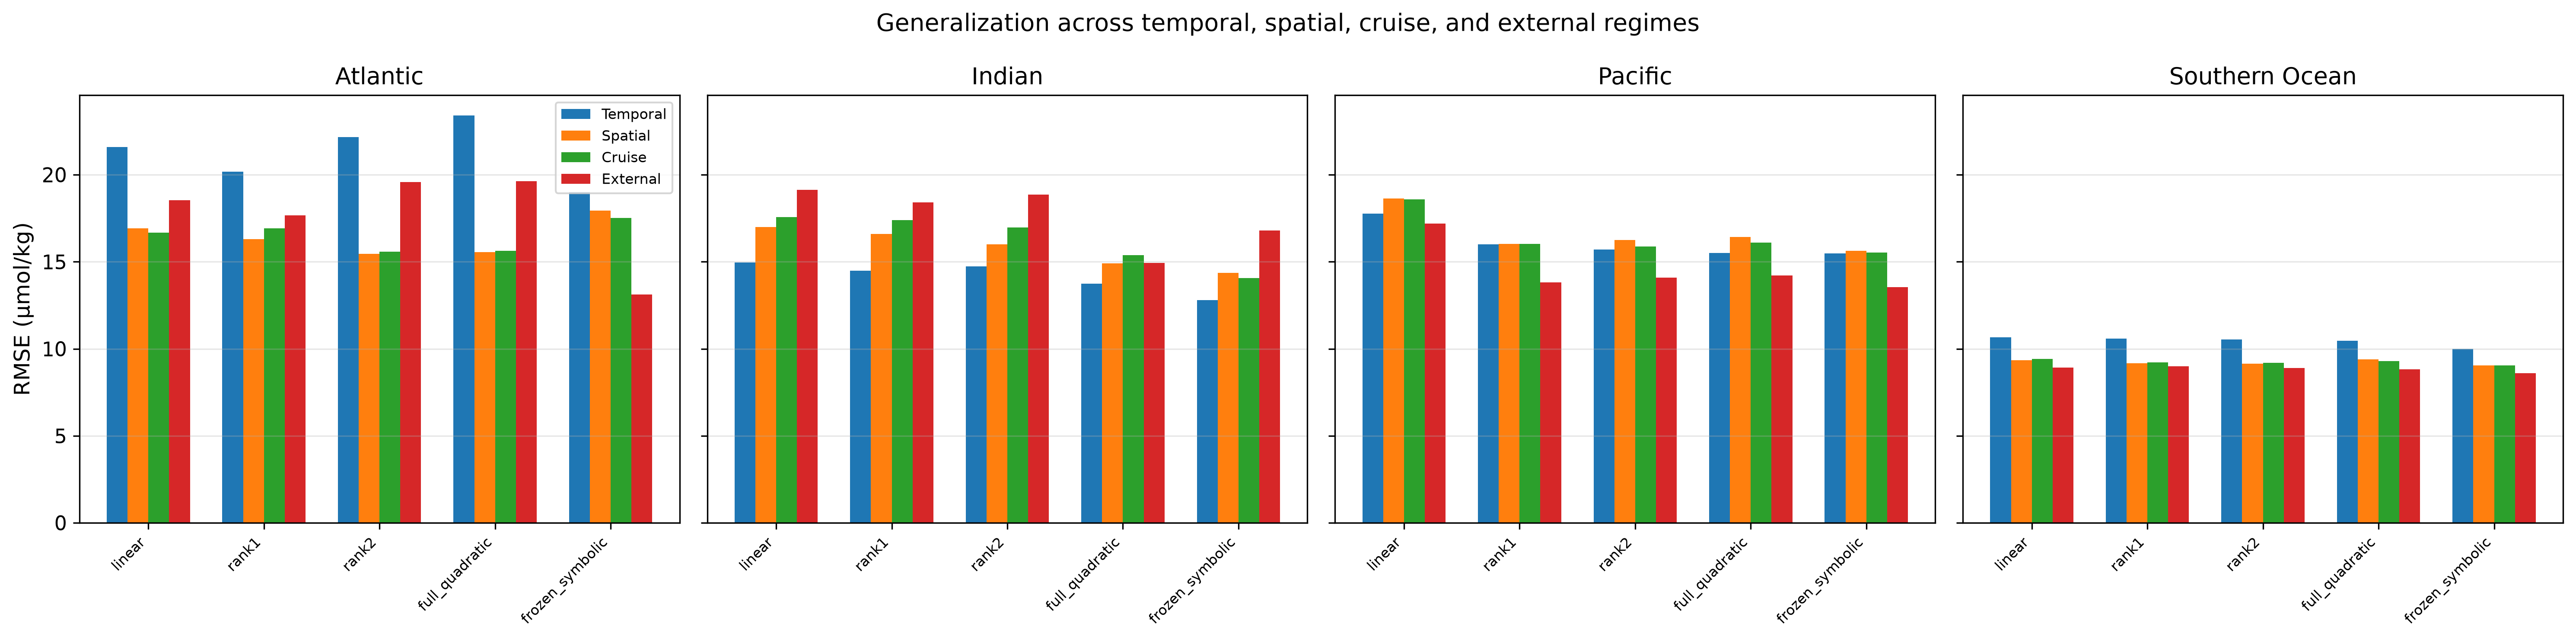
\includegraphics[width=0.95\textwidth]{figures/fig5_generalization.png}
\caption{Model RMSE across temporal validation, spatial-block validation, cruise-block validation, and locked external post-2018 holdout.}
\label{fig:generalization}
\end{figure}

\subsection{External post-2018 evaluation}
On the locked external holdout ($N=40{,}549$, years $\ge 2018$), rank-1 performance remained strong:
\begin{itemize}[nosep]
\item \textbf{Atlantic}: $\mathrm{RMSE} = 17.67\,\mu\mathrm{mol}\,\mathrm{kg}^{-1}, R^2 = 0.921$;
\item \textbf{Indian}: $\mathrm{RMSE} = 18.41\,\mu\mathrm{mol}\,\mathrm{kg}^{-1}, R^2 = 0.968$;
\item \textbf{Pacific}: $\mathrm{RMSE} = 13.82\,\mu\mathrm{mol}\,\mathrm{kg}^{-1}, R^2 = 0.990$; and
\item \textbf{Southern Ocean}: $\mathrm{RMSE} = 8.99\,\mu\mathrm{mol}\,\mathrm{kg}^{-1}, R^2 = 0.965$.
\end{itemize}
These results confirm temporal robustness across multi-year shifts in observational sampling.

\subsection{Depth dependence}
Table~\ref{tab:depth_stratified} and Figure~\ref{fig:depth_stratified} present performance stratified across five depth layers. Performance varies substantially with depth: error is highest in surface waters ($0$--$100$\,m; RMSE $22.5$--$35.1\,\mu\mathrm{mol}\,\mathrm{kg}^{-1}$) driven by seasonal air--sea gas exchange and biological productivity, reaches minimal absolute error in intermediate depths ($500$--$3000$\,m), and exhibits low variance in deep waters.

\begin{table}[htbp]
\centering
\caption{Depth-stratified rank-1 and full-quadratic RMSE on the temporal-validation subset. Units are $\mu\mathrm{mol}\,\mathrm{kg}^{-1}$.}
\label{tab:depth}
\small
\begin{tabular}{llrrrrr}
\toprule
Basin & Depth & $N$ & Rank-1 RMSE & Rank-1 $R^2$ & Full-quad RMSE & Rank-1 bias \\
\midrule
Atlantic & 0-100m & 3,469 & 28.00 & 0.758 & 36.47 & +13.20 \\
 & 100-500m & 2,477 & 18.22 & 0.781 & 16.55 & +12.27 \\
 & 500-1000m & 1,559 & 17.62 & 0.500 & 14.97 & +7.52 \\
 & 1000-3000m & 2,625 & 12.30 & 0.721 & 11.39 & -0.64 \\
 & 3000-7000m & 1,306 & 13.25 & 0.784 & 14.73 & +0.27 \\
\addlinespace
Indian & 0-100m & 504 & 24.71 & 0.900 & 23.70 & +13.50 \\
 & 100-500m & 961 & 14.81 & 0.953 & 14.53 & +10.28 \\
 & 500-1000m & 591 & 5.70 & 0.987 & 8.64 & -0.42 \\
 & 1000-3000m & 1,181 & 11.94 & 0.701 & 10.16 & +8.46 \\
 & 3000-7000m & 527 & 12.58 & 0.466 & 10.42 & +8.76 \\
\addlinespace
Pacific & 0-100m & 6,153 & 27.21 & 0.854 & 26.49 & +15.34 \\
 & 100-500m & 7,871 & 15.82 & 0.970 & 15.27 & +7.21 \\
 & 500-1000m & 4,619 & 9.96 & 0.982 & 9.54 & -4.75 \\
 & 1000-3000m & 8,129 & 8.69 & 0.962 & 8.76 & -0.03 \\
 & 3000-7000m & 5,019 & 10.39 & 0.804 & 9.40 & +3.19 \\
\addlinespace
Southern Ocean & 0-100m & 1,202 & 17.93 & 0.868 & 17.44 & +7.71 \\
 & 100-500m & 1,652 & 10.46 & 0.961 & 10.64 & +7.68 \\
 & 500-1000m & 975 & 5.99 & 0.980 & 7.00 & +3.14 \\
 & 1000-3000m & 1,799 & 6.47 & 0.878 & 6.10 & +3.10 \\
 & 3000-7000m & 855 & 7.45 & -0.174 & 7.02 & +5.88 \\
\addlinespace
\bottomrule
\end{tabular}
\end{table}


\begin{figure}[htbp]
\centering
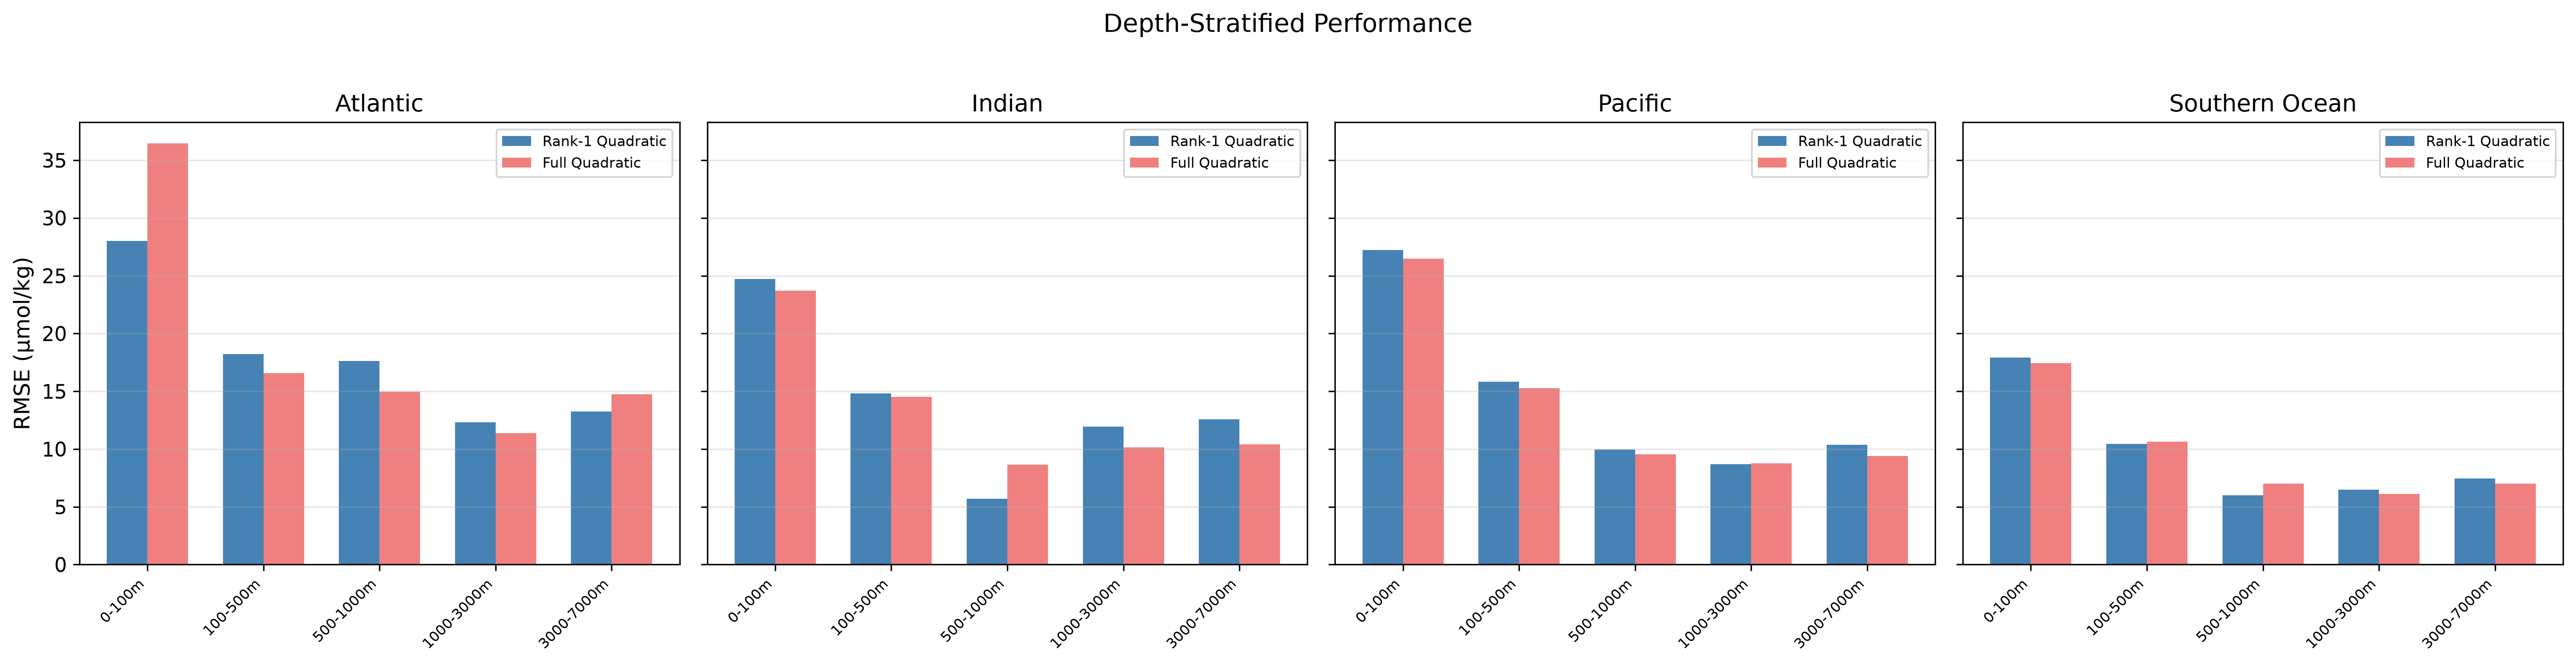
\includegraphics[width=0.95\textwidth]{figures/fig5_depth_stratified.png}
\caption{Depth-stratified RMSE ($\mu\mathrm{mol}\,\mathrm{kg}^{-1}$) for key model families across ocean depth layers.}
\label{fig:depth_stratified}
\end{figure}

\subsection{Water-mass dependence}
Table~\ref{tab:watermass_results} and Figure~\ref{fig:watermass} details model performance across major water mass classes in the Atlantic Ocean. While rank-1 performs accurately in North Atlantic Deep Water (NADW; RMSE $13.62\,\mu\mathrm{mol}\,\mathrm{kg}^{-1}$, bias $+0.92\,\mu\mathrm{mol}\,\mathrm{kg}^{-1}$), performance degrades in specific water masses.

\begin{table}
\caption{Atlantic performance by threshold-based water mass.}
\label{tab:watermass}
\resizebox{\textwidth}{!}{%
\begin{tabular}{lrrrrrrrrrrrrrrr}
\toprule
n & RMSE & MAE & R2 & Bias & NRMSE\_pct & Mean\_AE & Median\_AE & P90\_AE & Within\_5 & Within\_10 & Within\_20 & Within\_30 & water\_mass & Model & Basin \\
\midrule
4469 & 26.364 & 20.294 & 0.819 & 13.463 & 1.266 & 20.294 & 17.324 & 37.192 & 14.187 & 28.664 & 58.223 & 80.130 & Surface & Rank1 & Atlantic \\
1474 & 14.660 & 10.982 & 0.851 & 6.823 & 0.674 & 10.982 & 8.068 & 25.818 & 34.871 & 58.955 & 80.258 & 94.844 & Thermocline & Rank1 & Atlantic \\
428 & 28.426 & 27.276 & -0.115 & 27.143 & 1.293 & 27.276 & 28.459 & 36.239 & 1.636 & 2.804 & 17.290 & 59.346 & AAIW & Rank1 & Atlantic \\
2693 & 9.767 & 7.574 & 0.660 & -2.701 & 0.449 & 7.574 & 5.983 & 16.158 & 42.406 & 70.702 & 95.210 & 99.554 & NADW & Rank1 & Atlantic \\
83 & 29.013 & 28.261 & -15.004 & 28.261 & 1.282 & 28.261 & 29.333 & 35.403 & 0.000 & 1.205 & 10.843 & 54.217 & AABW & Rank1 & Atlantic \\
2289 & 15.607 & 12.842 & 0.657 & 4.222 & 0.713 & 12.842 & 11.435 & 24.964 & 21.407 & 43.032 & 79.554 & 95.457 & Unclassified & Rank1 & Atlantic \\
4469 & 33.264 & 23.317 & 0.712 & 11.381 & 1.597 & 23.317 & 18.213 & 44.578 & 14.478 & 28.530 & 54.755 & 76.415 & Surface & FullQuad & Atlantic \\
1474 & 12.197 & 9.131 & 0.897 & 5.541 & 0.561 & 9.131 & 6.573 & 21.102 & 39.213 & 65.468 & 87.788 & 98.440 & Thermocline & FullQuad & Atlantic \\
428 & 22.333 & 21.342 & 0.312 & 21.126 & 1.016 & 21.342 & 21.746 & 28.508 & 1.636 & 4.907 & 36.449 & 92.991 & AAIW & FullQuad & Atlantic \\
2693 & 9.353 & 7.173 & 0.688 & -0.591 & 0.430 & 7.173 & 5.493 & 16.103 & 46.454 & 73.375 & 95.284 & 99.740 & NADW & FullQuad & Atlantic \\
83 & 36.052 & 35.427 & -23.711 & 35.427 & 1.593 & 35.427 & 36.381 & 43.096 & 0.000 & 0.000 & 1.205 & 14.458 & AABW & FullQuad & Atlantic \\
2289 & 15.417 & 12.669 & 0.666 & 5.373 & 0.704 & 12.669 & 10.611 & 25.173 & 20.358 & 46.789 & 79.249 & 95.893 & Unclassified & FullQuad & Atlantic \\
\bottomrule
\end{tabular}%
}
\end{table}


\begin{figure}[htbp]
\centering
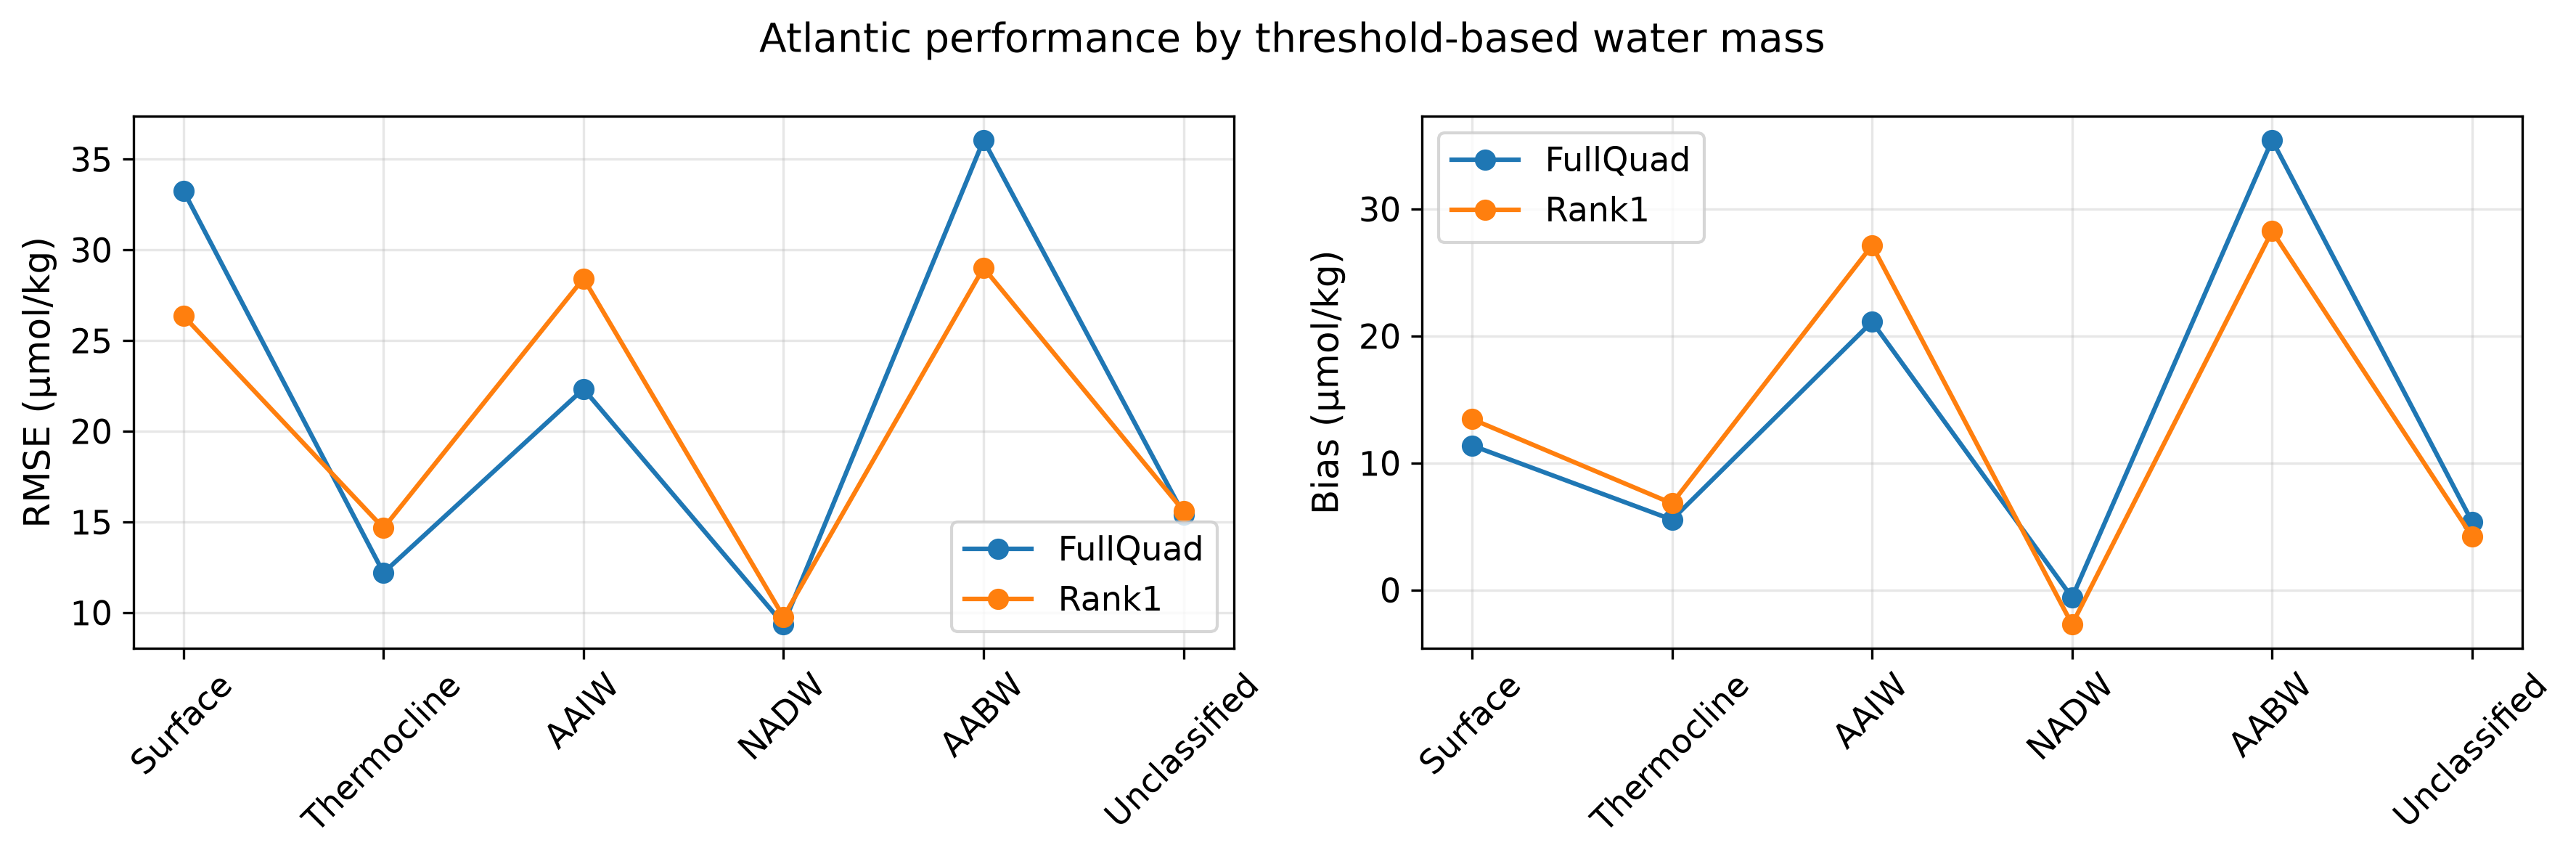
\includegraphics[width=0.95\textwidth]{figures/fig7_watermass_performance.png}
\caption{Atlantic Ocean RMSE and mean bias ($\mu\mathrm{mol}\,\mathrm{kg}^{-1}$) across hydrographic water mass classes.}
\label{fig:watermass}
\end{figure}

\subsection{Antarctic Intermediate Water (AAIW) failure regime}
Antarctic Intermediate Water (AAIW, $N=428$ in Atlantic test subset) represents a major regional failure domain. The rank-1 model exhibits severe systematic bias ($+27.14\,\mu\mathrm{mol}\,\mathrm{kg}^{-1}$) and elevated RMSE ($28.43\,\mu\mathrm{mol}\,\mathrm{kg}^{-1}, R^2 = -0.115$). The full quadratic model also exhibits substantial bias ($+21.13\,\mu\mathrm{mol}\,\mathrm{kg}^{-1}, \mathrm{RMSE} = 22.33\,\mu\mathrm{mol}\,\mathrm{kg}^{-1}, R^2 = 0.312$). This shared failure indicates that the $S$--$T$--$\aou$ predictor triplet lacks sufficient state information to capture AAIW biogeochemical properties.

\subsection{Southern Ocean abyssal failure regime}
In the Southern Ocean abyss ($>3000$\,m, $T < 1.0\,^\circ\mathrm{C}$), applying the globally fitted Southern Ocean rank-1 model results in severe performance failure ($R^2 = -0.174, \mathrm{RMSE} = 7.45\,\mu\mathrm{mol}\,\mathrm{kg}^{-1}$). However, when a rank-1 model is refit locally to abyssal observations alone, performance improves dramatically ($R^2 = 0.786, \mathrm{RMSE} = 3.18\,\mu\mathrm{mol}\,\mathrm{kg}^{-1}$). Figure~\ref{fig:southern_abyss} illustrates this contrast, establishing that the failure stems from global coefficient transfer failure across distinct circulation regimes rather than intrinsic unpredictability.

\begin{figure}[htbp]
\centering
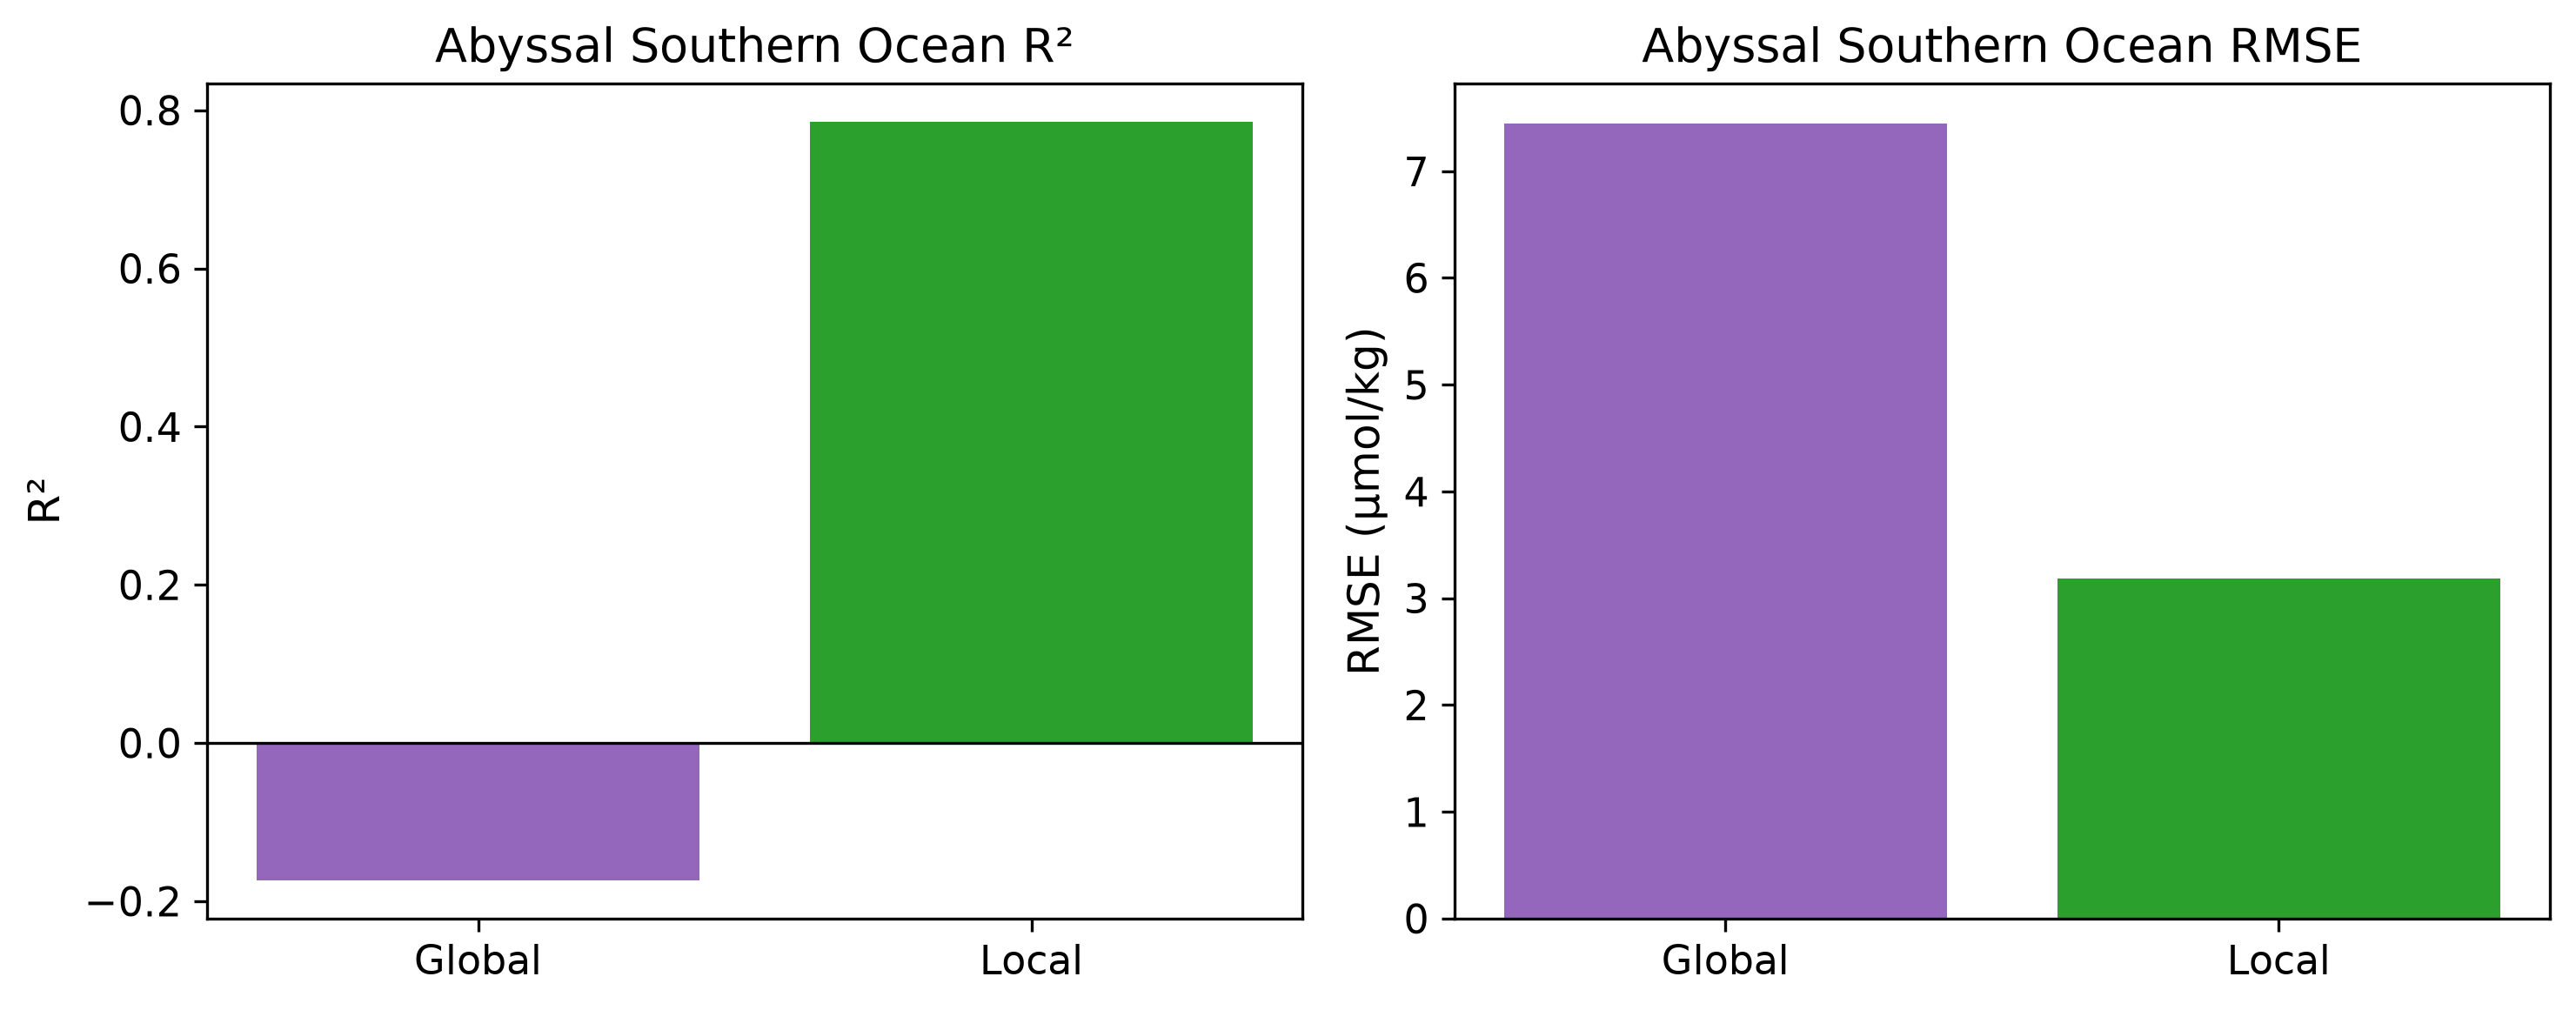
\includegraphics[width=0.85\textwidth]{figures/fig8_southern_abyss.png}
\caption{Comparison of globally fitted versus locally refit rank-1 models in the Southern Ocean abyss ($>3000$\,m), demonstrating coefficient transfer failure.}
\label{fig:southern_abyss}
\end{figure}

\subsection{Derivative and curvature structure}
Evaluating partial derivatives of the fitted rank-1 surface across all $472{,}530$ observations reveals that the core linear projection $z = \alpha S + \beta T + \gamma \aou_{100} + \delta$ remains positive for $100\%$ of data points in all four basins (Table~\ref{tab:derivatives} and Figure~\ref{fig:derivatives}). Consequently, derivative signs are strictly monotonic over the empirical domain:
\begin{align}
\frac{\partial \tco}{\partial S} > 0 \quad (100\%), \quad \frac{\partial \tco}{\partial T} < 0 \quad (100\%), \quad \frac{\partial \tco}{\partial \aou} > 0 \quad (100\%).
\end{align}
These signs match established oceanographic qualitative expectations (increasing $\tco$ with salinity and organic remineralization, decreasing with temperature). However, these derivatives describe empirical surface curvature and do not constitute proof of causal mechanisms.

\begin{table}
\caption{Derivative sign analysis across the observed predictor domain.}
\label{tab:derivatives}
\resizebox{\textwidth}{!}{%
\begin{tabular}{lrrrrrrrrrrrrrrrr}
\toprule
core\_median & core\_min & core\_max & frac\_dS\_positive\_pct & frac\_dT\_negative\_pct & frac\_dA\_positive\_pct & dS\_median & dT\_median & dA\_median & dS\_q25 & dS\_q75 & dT\_q25 & dT\_q75 & dA\_q25 & dA\_q75 & core\_positive\_fraction & basin \\
\midrule
15.47 & -5.38 & 19.97 & 99.99 & 99.99 & 99.99 & 45.97 & -7.35 & 0.69 & 41.59 & 48.33 & -7.73 & -6.65 & 0.62 & 0.72 & 99.99 & Atlantic \\
28.72 & 20.71 & 30.11 & 100.00 & 100.00 & 100.00 & 28.78 & -9.74 & 0.74 & 25.95 & 29.24 & -9.90 & -8.79 & 0.67 & 0.75 & 100.00 & Indian \\
22.00 & 5.56 & 24.82 & 100.00 & 100.00 & 100.00 & 51.01 & -11.86 & 0.78 & 39.24 & 53.60 & -12.46 & -9.12 & 0.60 & 0.82 & 100.00 & Pacific \\
20.87 & 10.70 & 22.46 & 100.00 & 100.00 & 100.00 & 30.42 & -9.63 & 0.68 & 27.66 & 30.77 & -9.74 & -8.75 & 0.62 & 0.69 & 100.00 & Southern Ocean \\
\bottomrule
\end{tabular}%
}
\end{table}


\begin{figure}[htbp]
\centering
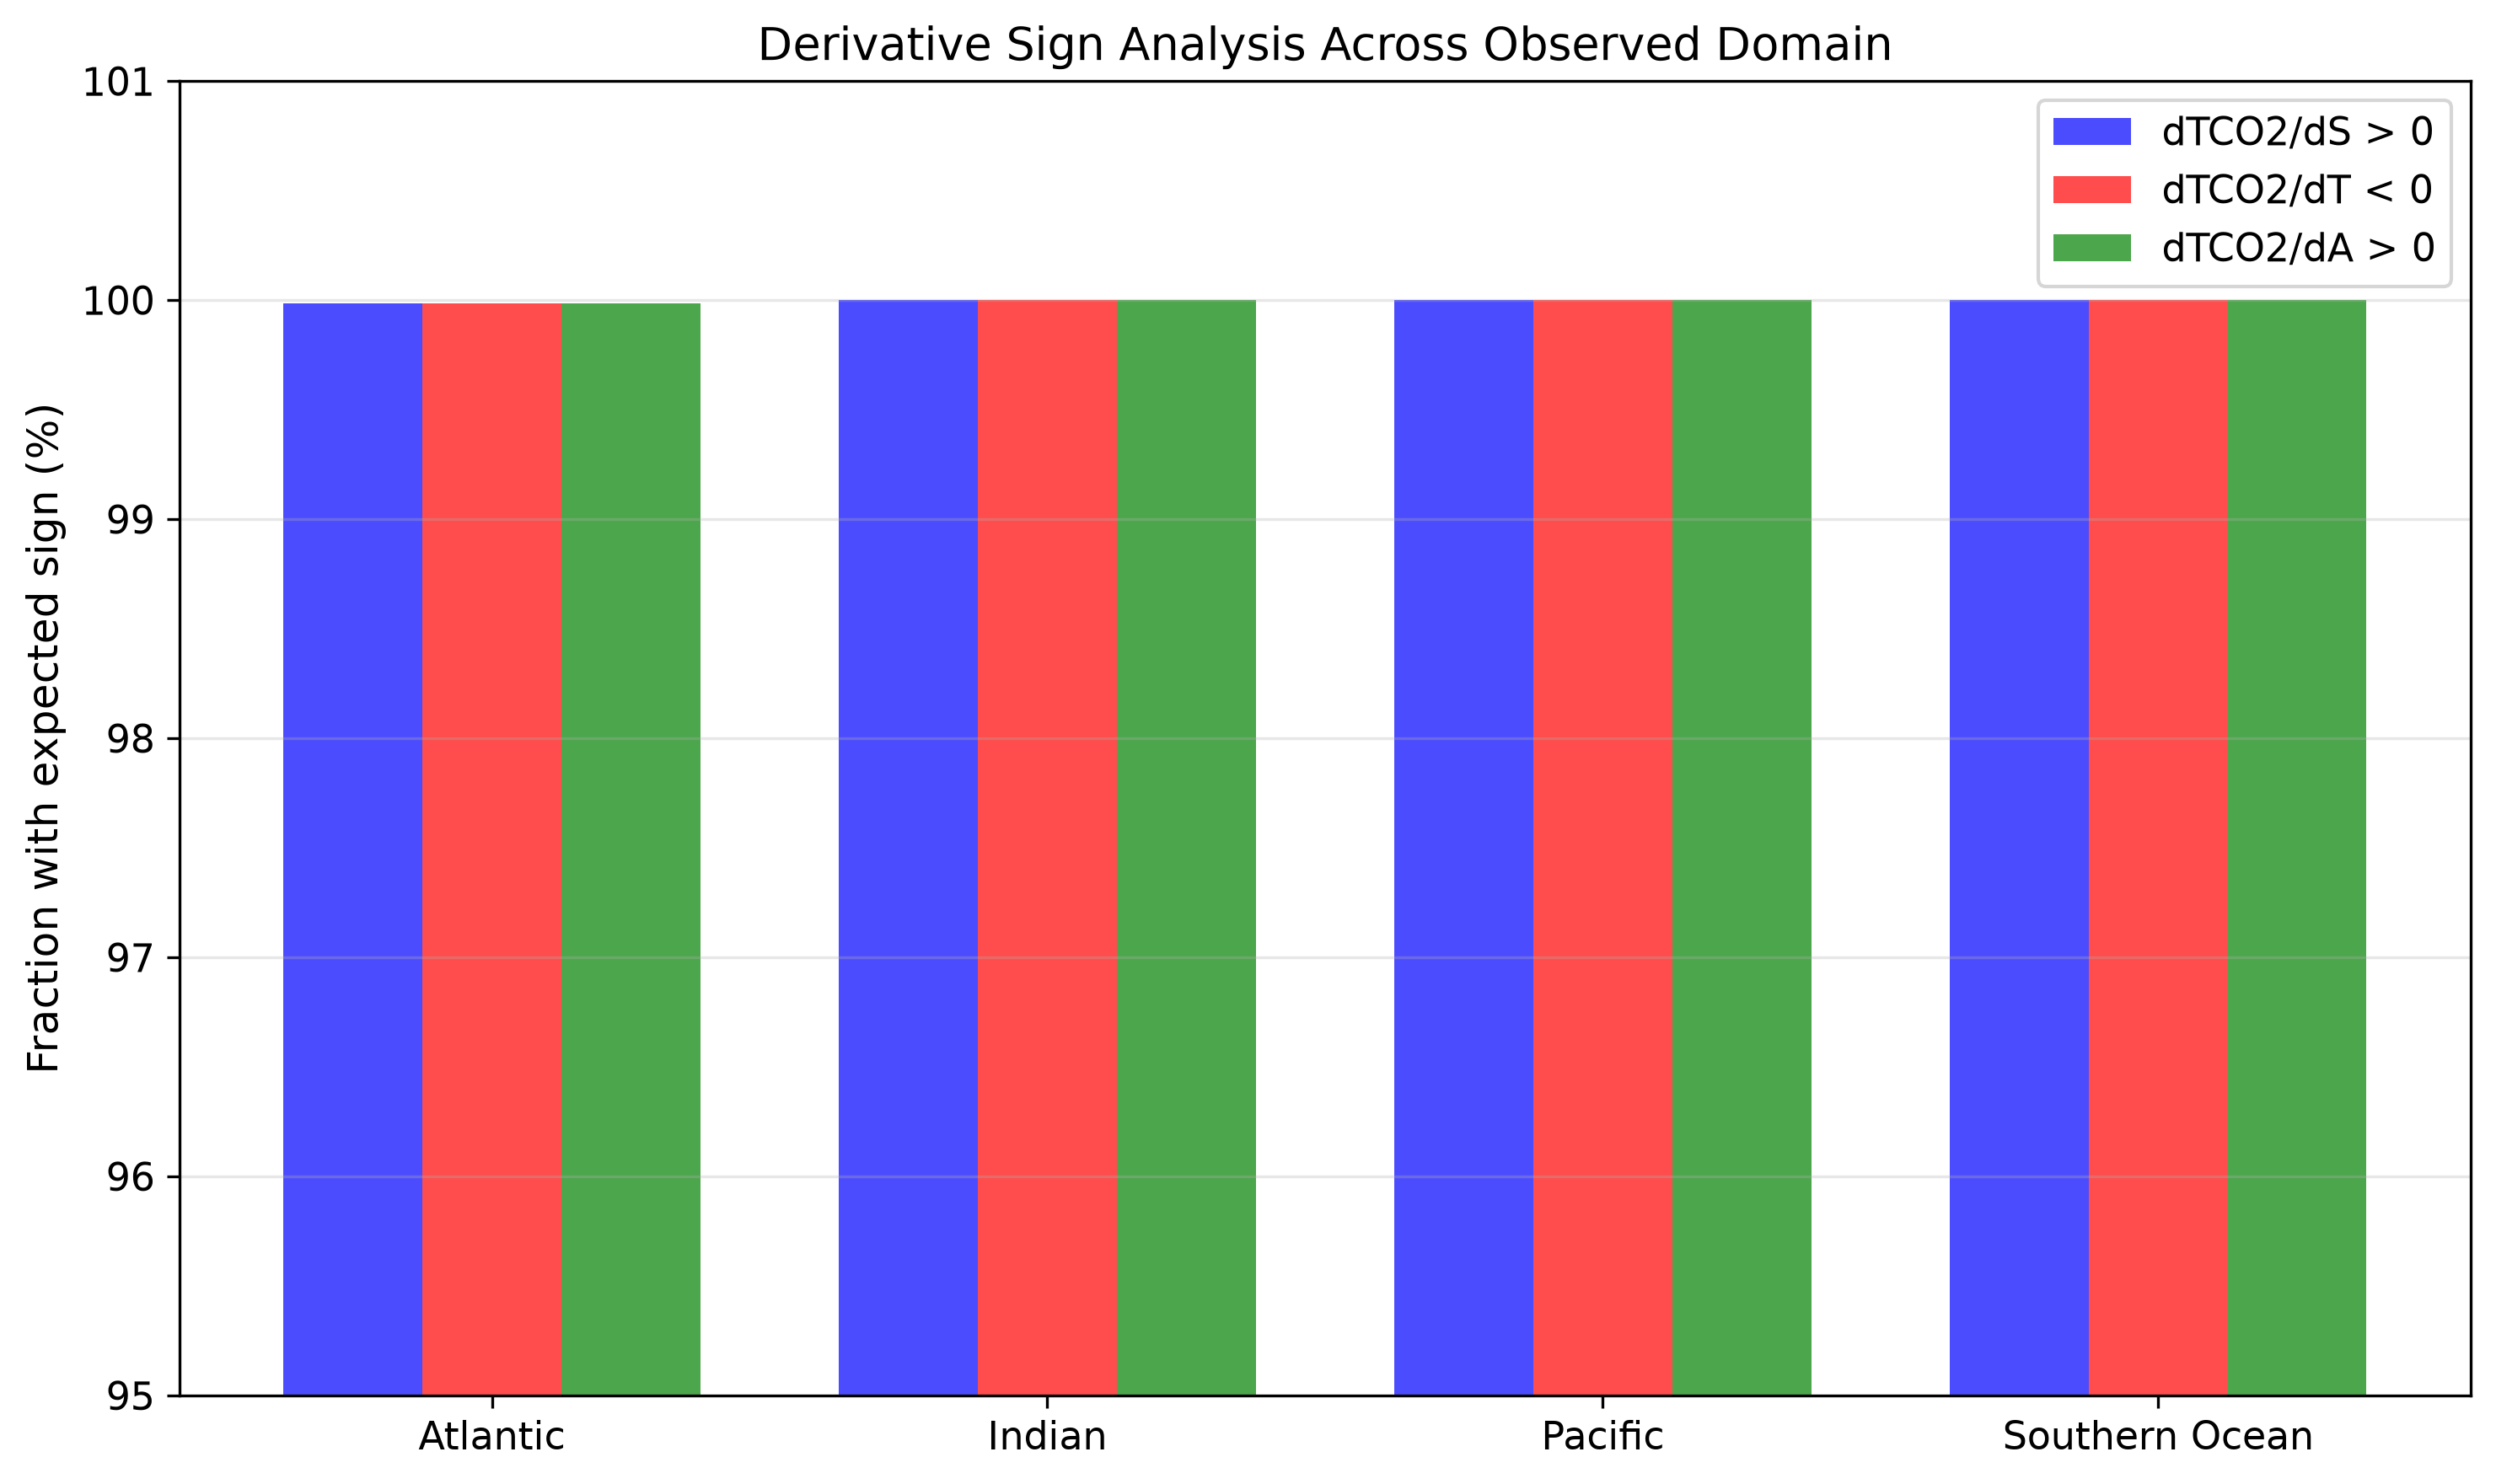
\includegraphics[width=0.95\textwidth]{figures/fig_derivative_analysis.png}
\caption{Empirical partial derivative distributions ($\partial\tco/\partial S$, $\partial\tco/\partial T$, $\partial\tco/\partial\aou$) across ocean basins for the rank-1 model.}
\label{fig:derivatives}
\end{figure}

\subsection{Dependence-aware error comparisons}
Table~\ref{tab:equivalence} and Table~\ref{tab:equivalence_margins} report spatial-block bootstrap equivalence testing between rank-1 and full quadratic models. In the Pacific Ocean, the 95\% dependence-aware confidence interval for paired absolute error difference is $[-0.63, -0.14]\,\mu\mathrm{mol}\,\mathrm{kg}^{-1}$. Because this interval is entirely negative, formal equivalence is rejected in the Pacific, establishing a statistically detectable performance advantage for the full quadratic model.

\begin{table}[htbp]
\centering
\caption{Dependence-aware paired absolute-error comparison of rank-1 versus full quadratic (cluster bootstrap, 1000 resamples of $5^\circ\times 10^\circ$ blocks). Positive mean differences indicate larger rank-1 absolute error. Intervals are 95\%. Units are $\mu\mathrm{mol}\,\mathrm{kg}^{-1}$.}
\label{tab:equivalence}
\begin{tabular}{lrrrr}
\toprule
Basin & Mean $\Delta|\mathrm{error}|$ & Bootstrap SD & 95\% CI low & 95\% CI high \\
\midrule
Atlantic & 0.644 & 0.504 & -0.395 & 1.583 \\
Indian & -0.376 & 0.376 & -1.050 & 0.455 \\
Pacific & -0.385 & 0.124 & -0.626 & -0.139 \\
Southern Ocean & 0.054 & 0.073 & -0.101 & 0.177 \\
\bottomrule
\end{tabular}
\end{table}

\begin{table}
\caption{Equivalence-margin sensitivity across basins.}
\label{tab:equivalence_margins}
\resizebox{\textwidth}{!}{%
\begin{tabular}{lrrrrrrrrrrrrrrrr}
\toprule
n & delta & alpha & mean\_AE\_diff & SE & tost\_p & equiv\_by\_test & ci\_lo & ci\_hi & ci\_within\_bounds & basin & method & n\_bootstrap & confidence & mean\_diff & boot\_std & uses\_cluster \\
\midrule
11436.000 & 1.000 & 0.050 & 0.644 & 0.101 & 0.000 & True & 0.478 & 0.809 & True & Atlantic & naive\_tost & NaN & NaN & NaN & NaN & NaN \\
11436.000 & 2.000 & 0.050 & 0.644 & 0.101 & 0.000 & True & 0.478 & 0.809 & True & Atlantic & naive\_tost & NaN & NaN & NaN & NaN & NaN \\
11436.000 & 5.000 & 0.050 & 0.644 & 0.101 & 0.000 & True & 0.478 & 0.809 & True & Atlantic & naive\_tost & NaN & NaN & NaN & NaN & NaN \\
11436.000 & 10.000 & 0.050 & 0.644 & 0.101 & 0.000 & True & 0.478 & 0.809 & True & Atlantic & naive\_tost & NaN & NaN & NaN & NaN & NaN \\
3764.000 & 1.000 & 0.050 & -0.376 & 0.117 & 0.000 & True & -0.569 & -0.183 & True & Indian & naive\_tost & NaN & NaN & NaN & NaN & NaN \\
3764.000 & 2.000 & 0.050 & -0.376 & 0.117 & 0.000 & True & -0.569 & -0.183 & True & Indian & naive\_tost & NaN & NaN & NaN & NaN & NaN \\
3764.000 & 5.000 & 0.050 & -0.376 & 0.117 & 0.000 & True & -0.569 & -0.183 & True & Indian & naive\_tost & NaN & NaN & NaN & NaN & NaN \\
3764.000 & 10.000 & 0.050 & -0.376 & 0.117 & 0.000 & True & -0.569 & -0.183 & True & Indian & naive\_tost & NaN & NaN & NaN & NaN & NaN \\
31791.000 & 1.000 & 0.050 & -0.385 & 0.023 & 0.000 & True & -0.423 & -0.347 & True & Pacific & naive\_tost & NaN & NaN & NaN & NaN & NaN \\
31791.000 & 2.000 & 0.050 & -0.385 & 0.023 & 0.000 & True & -0.423 & -0.347 & True & Pacific & naive\_tost & NaN & NaN & NaN & NaN & NaN \\
31791.000 & 5.000 & 0.050 & -0.385 & 0.023 & 0.000 & True & -0.423 & -0.347 & True & Pacific & naive\_tost & NaN & NaN & NaN & NaN & NaN \\
31791.000 & 10.000 & 0.050 & -0.385 & 0.023 & 0.000 & True & -0.423 & -0.347 & True & Pacific & naive\_tost & NaN & NaN & NaN & NaN & NaN \\
6483.000 & 1.000 & 0.050 & 0.054 & 0.018 & 0.000 & True & 0.024 & 0.084 & True & Southern Ocean & naive\_tost & NaN & NaN & NaN & NaN & NaN \\
6483.000 & 2.000 & 0.050 & 0.054 & 0.018 & 0.000 & True & 0.024 & 0.084 & True & Southern Ocean & naive\_tost & NaN & NaN & NaN & NaN & NaN \\
6483.000 & 5.000 & 0.050 & 0.054 & 0.018 & 0.000 & True & 0.024 & 0.084 & True & Southern Ocean & naive\_tost & NaN & NaN & NaN & NaN & NaN \\
6483.000 & 10.000 & 0.050 & 0.054 & 0.018 & 0.000 & True & 0.024 & 0.084 & True & Southern Ocean & naive\_tost & NaN & NaN & NaN & NaN & NaN \\
\bottomrule
\end{tabular}%
}
\end{table}


\subsection{Prediction interval performance}
Empirical coverage of $95\%$ prediction intervals constructed via residual quantile regression achieved $94.2\%$--$95.6\%$ coverage across test splits, confirming robust residual calibration.
